\documentclass[journal=jcim,manuscript=article]{achemso}

\usepackage[version=3]
{mhchem} % Formula subscripts using \ce{}

\usepackage{listings}
\usepackage{hyperref}
\usepackage{xr-hyper}
\usepackage{natbib}
\usepackage[newfloat]{minted}
\usepackage{multirow}

\externaldocument{SI}
% \documentclass[journal=jcim,manuscript=article]{achemso}
\usepackage{amsmath}
\usepackage{graphicx}
\usepackage{hyperref}
\usepackage[table,xcdraw]{xcolor}
\usepackage[left=1.5cm, right=1cm]{geometry}


\makeatletter
\let\oldminipage\minipage
\let\oldendminipage\endminipage
\renewenvironment{minipage}[1]{}{}
\g@addto@macro{\maketitle}{\let\minipage\oldminipage\let\endminipage\oldendminipage}
\makeatother


% fix some achemso rubbish
\renewcommand{\titlesize}{\normalsize}
\renewcommand{\affilsize}{\footnotesize	}
\renewcommand{\authorsize}{\footnotesize	}
\renewcommand{\emailsize}{\footnotesize}

%% Main manuscript contributors
\author{Hugo MacDermott-Opeskin}
\affiliation{Open Molecular Software Foundation, Davis CA, USA}
\author{Jenke Scheen}
\affiliation{Open Molecular Software Foundation, Davis CA, USA}
\author{Cas Wognum}
\affiliation{Valence Labs, Montréal, Québec, Canada}
\altaffiliation{Recursion Pharmaceuticals, Salt Lake City, UT, USA}
\author{Joshua, T Horton}
\affiliation{Open Molecular Software Foundation, Davis CA, USA}
\author{Devany West}
\affiliation{Open Molecular Software Foundation, Davis CA, USA}
\author{Alexander Matthew Payne}
\affiliation{Computational and Systems Biology Program, Memorial Sloan Kettering Cancer Center, New York, NY, USA}
\altaffiliation{Tri-Institutional PhD Program in Chemical Biology, Memorial Sloan Kettering Cancer Center, New York, NY, USA}
\author{Maria A Castellanos}
\affiliation{Computational and Systems Biology Program, Memorial Sloan Kettering Cancer Center, New York, NY, USA}
\author{Sean Colby}
\affiliation{Open Molecular Software Foundation, Davis CA, USA}

%% ASAP %%
\author{Edward Griffen}
\affiliation{MedChemica Consultancy Ltd, Macclesfield, UK}
\author{David Cousins}
\affiliation{MedChemica Consultancy Ltd, Macclesfield, UK}
\author{Jessica Stacey}
\affiliation{MedChemica Consultancy Ltd, Macclesfield, UK}
\author{Jasmin Cara Aschenbrenner}
\affiliation{Diamond Light Source, Didcot, UK}
\author{Daren Fearon}
\affiliation{Diamond Light Source, Didcot, UK}
\author{Blake Balcomb}
\affiliation{Diamond Light Source, Didcot, UK}
\author{Peter Marples}
\affiliation{Diamond Light Source, Didcot, UK}
\author{Charles W.E. Tomlinson}
\affiliation{Diamond Light Source, Didcot, UK}
\author{Ryan Lithgo}
\affiliation{Diamond Light Source, Didcot, UK}
\author{Max Winokan}
\affiliation{Diamond Light Source, Didcot, UK}
\author{Haim Barr}
\affiliation{Weizmann Institute of Science, Rehovot, IL}
\author{Noa Lahav}
\affiliation{Weizmann Institute of Science, Rehovot, IL}
\author{Gwendolyn Fate}
\affiliation{Thames Pharma Partners, USA}
\author{Bruce Lefker}
\affiliation{Thames Pharma Partners, USA}
\author{Ralph Robinson}
\affiliation{Thames Pharma Partners, USA}
\author{Tamas Szommer}
\affiliation{Centre for Medicines Discovery, Oxford, UK}
\author{Nick Lynch}
\affiliation{Curlew Research, UK}


%% OpenADMET
\author{Ryan Renslow}
\affiliation{Open Molecular Software Foundation, Davis CA, USA}
\author{Mallory Tollefson}
\affiliation{Open Molecular Software Foundation, Davis CA, USA}
\author{Cynthia Xu}
\affiliation{Open Molecular Software Foundation, Davis CA, USA}

% Valence 
\author{Jonny Hsu}
\affiliation{Valence Labs, Montréal, Québec, Canada}
\altaffiliation{Recursion Pharmaceuticals, Salt Lake City, UT, USA}
\author{Julien St-Laurent}
\affiliation{Valence Labs, Montréal, Québec, Canada}
\altaffiliation{Recursion Pharmaceuticals, Salt Lake City, UT, USA}
\author{Honore Etsmoberg}
\affiliation{Valence Labs, Montréal, Québec, Canada}
\altaffiliation{Recursion Pharmaceuticals, Salt Lake City, UT, USA}
\author{Lu Zhu}
\affiliation{Valence Labs, Montréal, Québec, Canada}
\altaffiliation{Recursion Pharmaceuticals, Salt Lake City, UT, USA}
\author{Andrew Quirke}
\affiliation{Valence Labs, Montréal, Québec, Canada}
\altaffiliation{Recursion Pharmaceuticals, Salt Lake City, UT, USA}

%% Participants
% All participants excluding the authors already listed in the main document
\author{Mohamed Iliyas Abdul Haleem}

\author{Irfan Alibay}
\affiliation{Open Molecular Software Foundation, Davis CA, USA}

\author{Gunjan Baid}
\affiliation{Inductive Bio, New York, NY, USA}

\author{Benjamin Birnbaum}
\affiliation{Inductive Bio, New York, NY, USA}

\author{Kevin Bishop}
\affiliation{Ontario Institute for Cancer Research, Toronto, ON, Canada}

\author{Hugo Bohorquez}
\affiliation{Ontario Institute for Cancer Research, Toronto, ON, Canada}

\author{Ashmita Bose}
\affiliation{University of Luxembourg, Luxembourg City, Luxembourg}

\author{C.J. Brown}
\affiliation{Alpha29, LLC}

\author{Jackson Burns}
\affiliation{MIT, Cambridge, MA, USA}

\author{Lianjin Cai}
\affiliation{University of Pittsburgh, Pittsburgh, PA, USA}

\author{Ruel Cedeno}
\affiliation{Novalix, 67000 Strasbourg, France}

\author{Vladimir Chupakhin}
\affiliation{Simulations Plus, Research Triangle Park, NC, USA}

\author{Finlay Clark}
\affiliation{Newcastle University, Newcastle, UK}

\author{Daniel Cole}
\affiliation{Newcastle University, Newcastle, UK}

\author{Carles Corbi-Verge}
\affiliation{Recursion, Salt Lake City, UT, USA}

\author{Muhammad Danial}
\affiliation{Shenzhen Institute of Synthetic Biology, Shenzhen Institutes of Advanced Technology, Chinese Academy of Sciences, Shenzhen 518055, China}

\author{Alec Davi}
\affiliation{Owkin, New York, NY, USA}

\author{Wim Dehaen}
\affiliation{UCT Prague, Prague, Czech Republic}

\author{Niklas Piet Doering}
\affiliation{Freie Universität Berlin, Berlin, Germany}

\author{Alexis Dougha}
\affiliation{BFA, Université Paris Cité, CNRS UMR 8251, Inserm U1133, 75013 Paris, France}

\author{Bryce Eakin}
\affiliation{Inductive Bio, New York, NY, USA}

\author{Anatol Ehrlich}
\affiliation{University of Vienna, Vienna, Austria}

\author{Rokas Elijosius} % [Pending check]
\affiliation{University of Cambridge, Cambridge, UK}

\author{Jozef Fülöp}
\affiliation{UCT Prague, Prague, Czech Republic}

\author{Anthony Gitter}
\affiliation{University of Wisconsin-Madison, Madison, WI, USA}
\altaffiliation{Morgridge Institute for Research, Madison, WI, USA}

\author{Yaowen Gu}
\affiliation{New York University, New York, NY, USA}

\author{Teresa Head-Gordon}
\affiliation{University of California, Berkeley, CA, USA}

\author{Ellena Jiang}
\affiliation{University of Vienna, Vienna, Austria}

\author{Benjamin Kaminow}
\affiliation{Computational and Systems Biology Program, Memorial Sloan Kettering Cancer Center, New York, NY, USA}

\author{Sina Khosravi}
\affiliation{Mashhad University of Medical Sciences, Mashhad, Khorasan Razavi, Iran}

\author{Asma Feriel Khoualdi} % [Pending check]
\affiliation{Newcastle University, Newcastle, UK}

\author{Eelke Bart Lenselink}
\affiliation{Galapagos NV, 2800 Mechelen, Belgium}

\author{Zhirong Liu}
\affiliation{Peking University, Beijing, China}

\author{Yue Liu}
\affiliation{University of Pittsburgh, Pittsburgh, PA, USA}

\author{Sijie Liu}
\affiliation{Freie Universität Berlin, Berlin, Germany}

\author{Yizhou Ma}
\affiliation{QuantaBricks, Newark, NJ, USA}

\author{Patrick Maher}
\affiliation{Inductive Bio, New York, NY, USA}

\author{Imke Mayer} % [Pending Check]
\affiliation{Owkin, New York, NY, USA}

\author{Antonia Mey}
\affiliation{University of Edinburgh, Edinburgh, Scotland, UK}

\author{Floriane Montanari} % [Pending check]
\affiliation{Owkin, New York, NY, USA}

\author{Taoyu Niu}
\affiliation{University of Pittsburgh, Pittsburgh, PA, USA}

\author{Ryusei Ogino}
\affiliation{Japan Tobacco INC., Minato City, Tokyo, Japan}

\author{Ashok Palaniappan}
\affiliation{SASTRA Deemed University, Thanjavur, Tamil Nadu 613401, India}

\author{Xiaolin Pan}
\affiliation{New York University, New York, NY, USA}

\author{Auro Patnaik}
\affiliation{University of Edinburgh, Edinburgh, Scotland, UK}

\author{Long-Hung Pham}
\affiliation{Imperial College London, London, UK}

\author{Luis Pinto}
\affiliation{Independent Researcher}

\author{Justin Purnomo}
\affiliation{University of California, Berkeley, CA, USA}

\author{Alexander Rich}
\affiliation{Inductive Bio, New York, NY, USA}

\author{Lars Schaaf}
\affiliation{University of Cambridge, Cambridge, UK}

\author{Christoph Schran}
\affiliation{University of Cambridge, Cambridge, UK}

\author{Satya Pratik Srivastava}
\affiliation{Shiv Nadar University, Greater Noida, Uttar Pradesh, India}

\author{Kunyang Sun}
\affiliation{University of California, Berkeley, CA, USA}

\author{Zhaoxi Sun}
\affiliation{Shenzhen University of Advanced Technology, Shenzhen, China}

\author{Valerij Talagayev}
\affiliation{Freie Universität Berlin, Berlin, Germany}

\author{Balamurugan Thirukonda Subramanian Balakrishnan}

\author{Alexandre Tkatchenko}
\affiliation{University of Luxembourg, Luxembourg City, Luxembourg}

\author{Wojtek Treyde}
\affiliation{University of Oxford, Oxford, UK}

\author{Austin Tripp}
\affiliation{Valence Labs, Quebec, Canada}

\author{Nopsinth Vithayapalert}
\affiliation{VISTEC, Pa Yup Nai, Thailand}

\author{Yingze Wang}
\affiliation{University of California, Berkeley, CA, USA}

\author{Azmine Toushik Wasi}
\affiliation{Shahjalal University of Science and Technology, Sylhet, Bangladesh}

\author{Steffen Wedig}
\affiliation{University of Cambridge, Cambridge, UK}

\author{Bofei Xu}
\affiliation{Peking University, Beijing, China}

\author{Weijun Zhou}
\affiliation{New York University, New York, NY, USA}



%% ASAP PIs
\author{Frank von Delft}
\affiliation{Diamond Light Source, Didcot, UK}
\author{Alpha Lee}
\affiliation{PostEra, Cambridge, MA, USA}
\author{Karla Kirkegaard}
\affiliation{Stanford University School of Medicine: Stanford, CA, US}
\author{Peter Sjö}
\affiliation{Drugs for Neglected Diseases initiative: Geneva, Genève, CH}

%% OpenADMET PIs
\author{Sri Kosuri} 
\affiliation{Octant Inc: Emeryville, CA, US}

\author{James S. Fraser}
\affiliation{University of California San Francisco, San Francisco, CA, USA}

%% John as final as PI across both
\author{John D. Chodera}
\affiliation{Memorial Sloan Kettering Cancer Center, New York, NY, USA}

\email{*jenke.scheen@omsf.io}


% Title 
\title{Supplementary Materials: A Computational Community Blind Challenge on Pan-Coronavirus Drug Discovery Data}

\begin{document}

\maketitle

\begin{figure}
    
\includegraphics[scale=0.175]{04_figs_leaderboards/admet_endpoints.png}
    
\includegraphics[scale=0.175]{04_figs_leaderboards/admet_endpoints_log10.png}
  \caption{Distributions of ADMET endpoints for train (blue) and test (orange) show outlier and dynamic range difficulties.  HLM, MLM, and Permeability have long tails, KSOL, has mostly low and high values within this dynamic range.  Raw values (top) and log10 values (bottom).}
  \label{fgr:admet_endpoints}
\end{figure}

\begin{figure}
    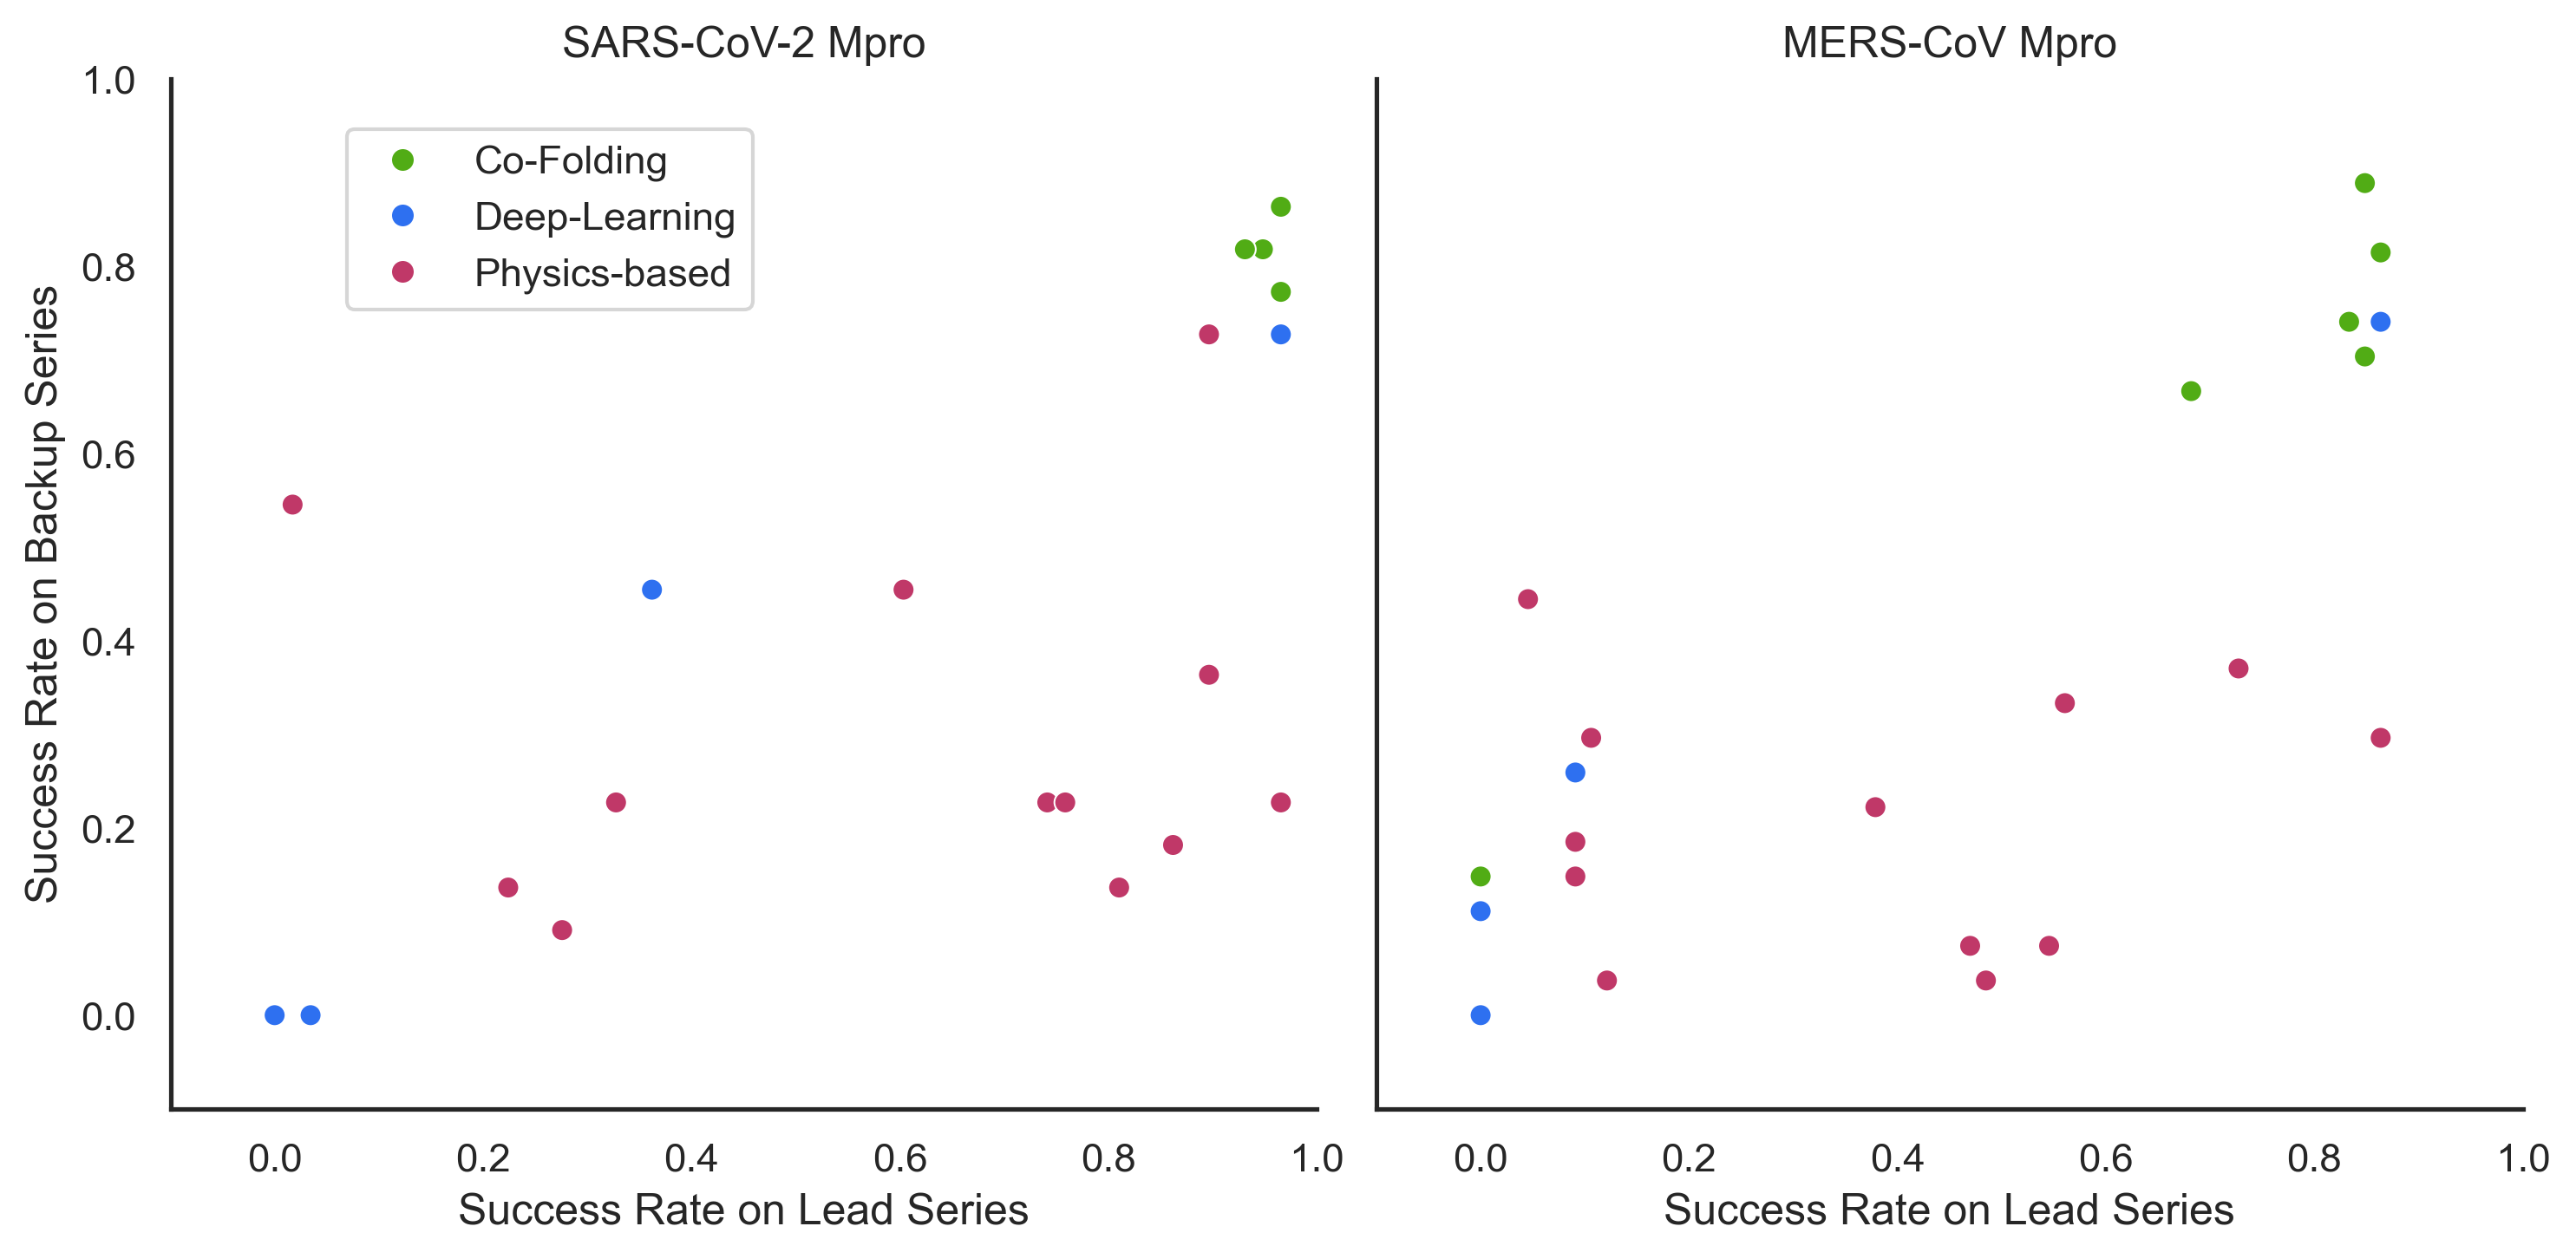
\includegraphics[scale=0.75]{04_figs_leaderboards/success_rate_lead_vs_backup_comparison.png}
  \caption{Success rates of each type of model on the lead series vs backup series. This shows that the worse performance on the backup series comes mainly from the physics-based models, with the co-folding models doing well on both and the deep-learning doing poorly on both.}
  \label{fgr:success_rate_lead_vs_backup}
\end{figure}

\begin{figure}
    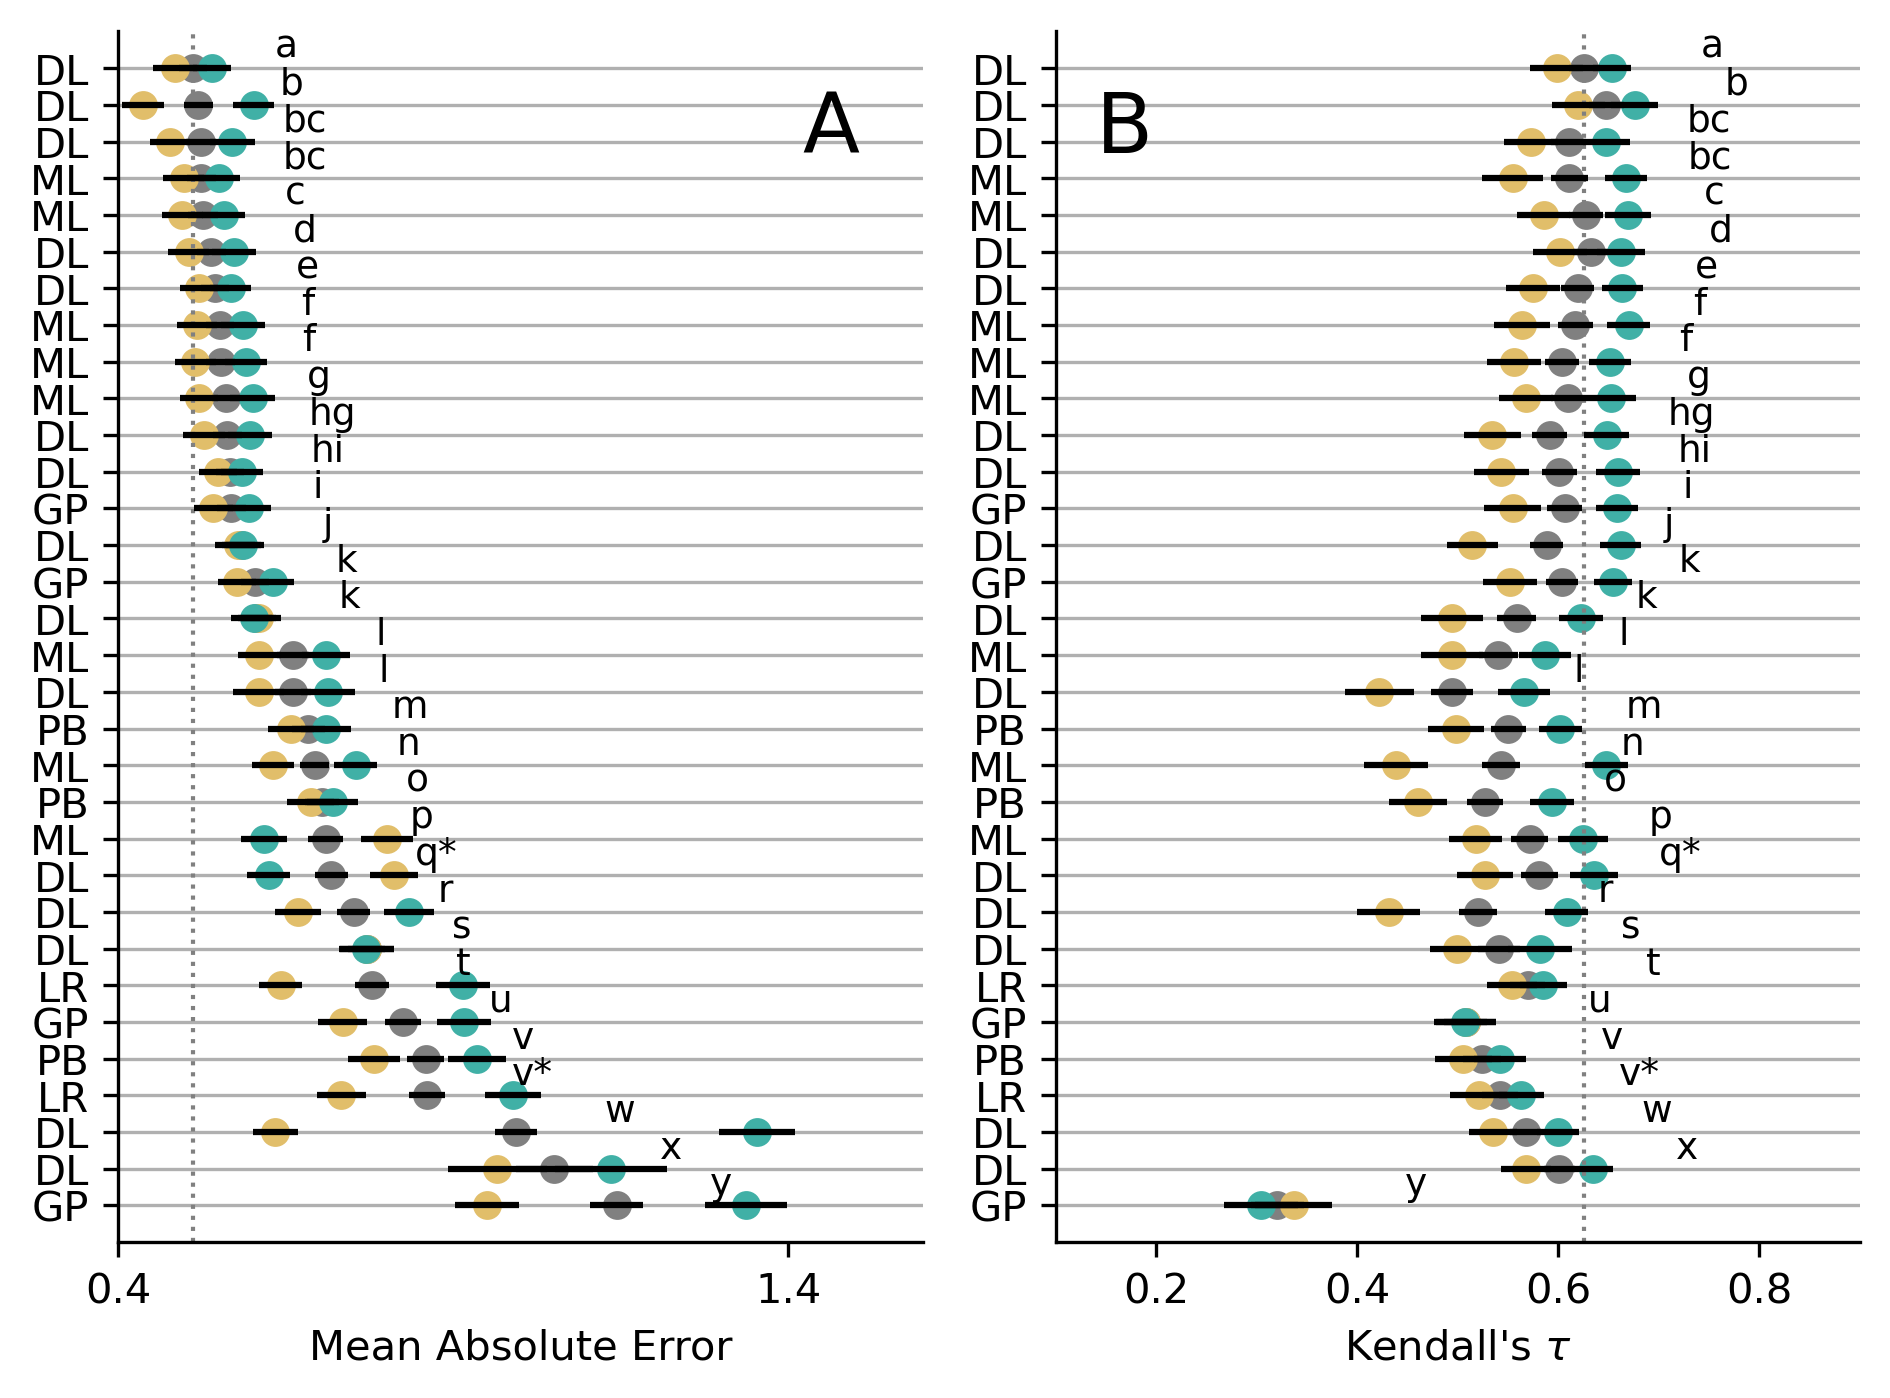
\includegraphics[scale=0.75]{SI/SI_potency_leaderboards.png}
  \caption{Participants performed diversely on potency predictions. A) leaderboard of the potency subchallenge as each entry's category (DL=Deep Learning, ML=Machine Learning, PB=Physics-Based, GP=Gaussian Process, LR=Linear Regression) and split by target; MERS-CoV Mpro in yellow, SARS-CoV-2 Mpro in green). B) replication of panel A but using the ranking metric \textit{kendall's $\tau$ }. Baseline models as deployed by the organizers are marked with asterisks. Each entry is annotated with its statistical ranking by the Compact Letter Display (CLD) system\cite{cld_algorithm_2004}.}
  \label{fgr:success_rate_lead_vs_backup}
\end{figure}

\end{document}


\newenvironment{code}{\captionsetup{type=listing}}{}

\newcommand*\mycommand[1]{\texttt{\emph{#1}}}

%%%%%%%%%%%%%%%%%%%%%%%%%%%%%%%%%%%%%%%%%%%%%%%%%%%%%%%%%%%%%%%%%%%%%
%% Meta-data block
%% ---------------
%% Each author should be given as a separate \author command.
%% Valence / Polaris 
\author{Hugo MacDermott-Opeskin}
\affiliation{Open Molecular Software Foundation, Davis CA, USA}
\author{Jenke Scheen}
\affiliation{Open Molecular Software Foundation, Davis CA, USA}
\author{Cas Wognum}
\affiliation{Valence Labs, Montréal, Québec, Canada}
\altaffiliation{Recursion Pharmaceuticals, Salt Lake City, UT, USA}
\author{Joshua, T Horton}
\affiliation{Open Molecular Software Foundation, Davis CA, USA}
\author{Devany West}
\affiliation{Open Molecular Software Foundation, Davis CA, USA}
\author{Alexander Matthew Payne}
\affiliation{Computational and Systems Biology Program, Sloan Kettering Institute, Memorial Sloan Kettering Cancer Center, New York, NY, USA}
\altaffiliation{Tri-Institutional PhD Program in Chemical Biology, Memorial Sloan Kettering Cancer Center, New York, NY, USA}
\author{Maria Castellanos}
\affiliation{Memorial Sloan Kettering Cancer Center, New York, NY, USA}
\author{Jonny Hsu}
\affiliation{Valence Labs, Montréal, Québec, Canada}
\altaffiliation{Recursion Pharmaceuticals, Salt Lake City, UT, USA}
\author{Andrew Quirke}
\affiliation{Valence Labs, Montréal, Québec, Canada}
\altaffiliation{Recursion Pharmaceuticals, Salt Lake City, UT, USA}
\author{Julien St-Laurent}
\affiliation{Valence Labs, Montréal, Québec, Canada}
\altaffiliation{Recursion Pharmaceuticals, Salt Lake City, UT, USA}
\author{Honore Etsmoberg}
\affiliation{Valence Labs, Montréal, Québec, Canada}
\altaffiliation{Recursion Pharmaceuticals, Salt Lake City, UT, USA}
\author{Lu Zhu}
\affiliation{Valence Labs, Montréal, Québec, Canada}
\altaffiliation{Recursion Pharmaceuticals, Salt Lake City, UT, USA}
\author{A whole bunch of participants}
\affiliation{Participants' author list: SI 1}
\author{A whole bunch of ASAP people}
\affiliation{ASAP' author list: SI 2}
\author{Externals}
\affiliation{Elsewhere}
\author{PIs?}
\affiliation{In charge}

\email{*hugo.macdermott-opeskin@omsf.io}

%%%%%%%%%%%%%%%%%%%%%%%%%%%%%%%%%%%%%%%%%%%%%%%%%%%%%%%%%%%%%%%%%%%%%
%% The document title should be given as usual. Some journals require
%% a running title from the author: this should be supplied as an
%% optional argument to \title.
%%%%%%%%%%%%%%%%%%%%%%%%%%%%%%%%%%%%%%%%%%%%%%%%%%%%%%%%%%%%%%%%%%%%%
\title{A Computational Community Blind Challenge on Pan-Coronavirus Drug Discovery Data}

\begin{document}

%%%%%%%%%%%%%%%%%%%%%%%%%%%%%%%%%%%%%%%%%%%%%%%%%%%%%%%%%%%%%%%%%%%%%
%% The abstract environment will automatically gobble the contents
%% if an abstract is not used by the target journal.
%%%%%%%%%%%%%%%%%%%%%%%%%%%%%%%%%%%%%%%%%%%%%%%%%%%%%%%%%%%%%%%%%%%%%
\begin{abstract}
Computational blind challenges offer critical, real-world assessment opportunities to enable scientific progress, as demonstrated by a breadth of breakthroughs over the last decade. We report the outcomes and key insights from an open science community blind challenge focused on antiviral drug discovery for coronaviruses, using lead optimization data from the ASAP Discovery Consortium, in partnership with Polaris and OpenADMET. This collaborative initiative invited global participants across academia and industry to develop and apply computational methods to predict the biochemical potency and crystallographic ligand poses of small molecules against key coronavirus targets, SARS-CoV-2 and MERS-CoV Mpro, as well as multiple absorption, distribution, metabolism and excretion (ADMET) assay endpoints—using undisclosed experimental datasets as benchmarks. By evaluating submissions across multiple tasks and compounds, we established performance leaderboards and conducted meta-analyses to assess methodological strengths, common pitfalls, and areas for improvement. This analysis provides a foundation for best practices in real-world machine learning evaluation, grounded in community-driven benchmarking. We also highlight how next-generation platforms such as Polaris (polarishub.io) enable rigorous challenge design, embedded evaluation frameworks, and broad community engagement. This paper synthesizes the collective findings of the challenge, offering a high-level overview of the data, evaluation infrastructure, and top-performing strategies. It provides context and support for the accompanying papers authored by the challenge participants in this special issue, which explore individual approaches in greater depth. Together, these contributions aim to advance reproducible, trustworthy, and high-impact machine learning in drug discovery, and to explore best practices and pitfalls in future blind challenge design and execution, including upcoming OpenADMET efforts.
\end{abstract}

%%%%%% MAKE THE WHOLE MANUSCRIPT DOUBLE COLUMN FOR EASIER FIGURE FORMATTING
% \twocolumn
%%%%%%%%%%%%%%%%%%%%%%%%%%%%%%%%%%%%%%%%%%%%%%%%%%%%%%%%%%%%%%%%%%%%%
%% INTRODUCTION
%%%%%%%%%%%%%%%%%%%%%%%%%%%%%%%%%%%%%%%%%%%%%%%%%%%%%%%%%%%%%%%%%%%%%
\section{Introduction}
%% DRUG DISCOVERY COMPCHEM DOESNT GET ENOUGH DATA FOR PROPER MODELS
Computational modeling for drug discovery is often hindered by data shortages, particularly in obtaining high-quality, diverse, and openly accessible datasets that explore chemical space in high detail around target-specific chemical series. Predictive models such as those used in structure-based drug design, molecular docking, and machine learning rely heavily on large volumes of high-quality experimental data to be effective. However, much of this data remains proprietary, fragmented or improperly reported, limiting model performance and reproducibility. Open science initiatives that provide access to comprehensive datasets will be crucial for advancing these models and improving their performance going forward. 
%% TO BUILD PROPER MODELS WE NEED PROPER BENCHMARKS AND CHALLENGES
Besides data availability, building sustainable and translatable computational models requires robust strategies to objectively compare different models. Community blind challenges provide a structured and unbiased framework for evaluating computational methods in drug discovery. Several notable community blind challenges have driven progress in computational drug discovery: 
The \textit{CACHE initiative}\cite{ackloo_al-awar_amaro_arrowsmith_azevedo_al._2022} evaluates hit-finding methods by experimentally testing predicted compounds in a fully open, prospective and standardized framework. The D3R Grand Challenges\cite{parks_gaieb_chiu_yang_shao_walters_jansen_mcgaughey_lewis_bembenek_et} benchmarked pose prediction and binding affinity ranking algorithms (e.g. free energy calculation methods) using small, focused blinded protein–ligand datasets. The Statistical Assessment of Modeling of Proteins and Ligands (SAMPL) series\cite{amezcua_setiadi_mobley_2024} involved evaluating model perfomance on a wide variety of physical properties, including partition coefficients, logD, pKa and ligand hydration free energies. Finally, the CASP competition\cite{andriy_kryshtafovych_schwede_topf_krzysztof_2019} challenges participants to predict protein structures \textit{ a priori}, with famous breakthroughs such as AlphaFold2 and RoseTTAFold transforming the computational drug discovery field.\cite{jumper_evans_pritzel_green_figurnov_ronneberger_tunyasuvunakool_bates_žídek_2021, baek_2021} However, most blind challenges to date have involved single-modality data sets aggregated across drug discovery projects, and often between different drug discovery institutions and organizations. This creates a major gap in benchmarking how well current models perform on 'real-world' drug discovery problems that focus on a single project (i.e., involving the development of therapies against a defined biological target) and span multiple modalities. 
%% ASAP DISCOVERY RAN AS OPEN SCIENCE AND APPROACHED PRECLINICAL CANDIDATE DISCLOSURE MILESTONE - PERFECT OPPORTUNITY
During the SARS-CoV-2 pandemic the COVID Moonshot consortium\cite{boby_2023} demonstrated the feasibility of developing a straight-to-generic main protease (Mpro) inhibitor in record time using an open science approach. Building on this success, the AI-Driven Structure-enabled Antiviral Platform (ASAP) Discovery Consortium was launched as part of the NIH AViDD program, leveraging structure-enabled and artificial intelligence approaches, alongside a global team of experts, to advance structural biology, medicinal chemistry, biochemistry, and pre-clinical development for antiviral drug discovery. One of the main pillars of ASAP is its commitment to global accessibility of antivirals through an equitable licensing structure\cite{griffen_2024}. ASAP's open science approach requires regular disclosure of project data into the public domain (with some limitations around bleeding edge lead-opt data), however, with ASAP's pan-coronavirus program (targeting SARS-CoV-2 and MERS-CoV Mpro) approaching a preclinical candidate disclosure in March 2025 (now disclosed)\cite{griffen_2025_acs}, a significant portion of its drug discovery data was withheld to ensure a successful patent application within ASAP's equitable-access IP framework. This presented a unique opportunity to host a computational community blind challenge using the withheld dataset spanning multiple drug discovery modalities.

%% PARTNERSHIP WITH POLARIS AND OPENADMET%%
Running a computational blind challenge requires significant community engagement, technical expertise, and robust evaluation procedures. To this end, ASAP partnered with Valence Labs who have developed Polaris, an open platform to enable easy access to drug discovery datasets and benchmarks. Polaris provides robust challenge infrastructure, dataset hosting and expertise in best practices in model evaluation. Additionally, ASAP partnered with the team at OpenADMET, a new ARPA-H funded project under the Open Molecular Software Foundation (OMSF) focused on machine learning for ADMET modeling. The blind challenge developed between these partners will from now on be referred to as the ASAP-Polaris-OpenADMET antiviral competition. 
%% QUICK DESCRIPTION OF WHAT DATA WAS IN THE CHALLENGE
The bulk of the dataset used in the challenge consisted of lead optimization (leadopt) data, selected to mirror the challenges faced by ASAP during its own leadopt campaign. To this end, three subtasks or \textit{sub-challenges} were designed in three modalities common to drug discovery: 1) crystallographic ligand pose prediction, 2) biochemical potency prediction, and 3) ADMET endpoint prediction (figure \ref{fgr:datasets_overview}).


\begin{figure}
    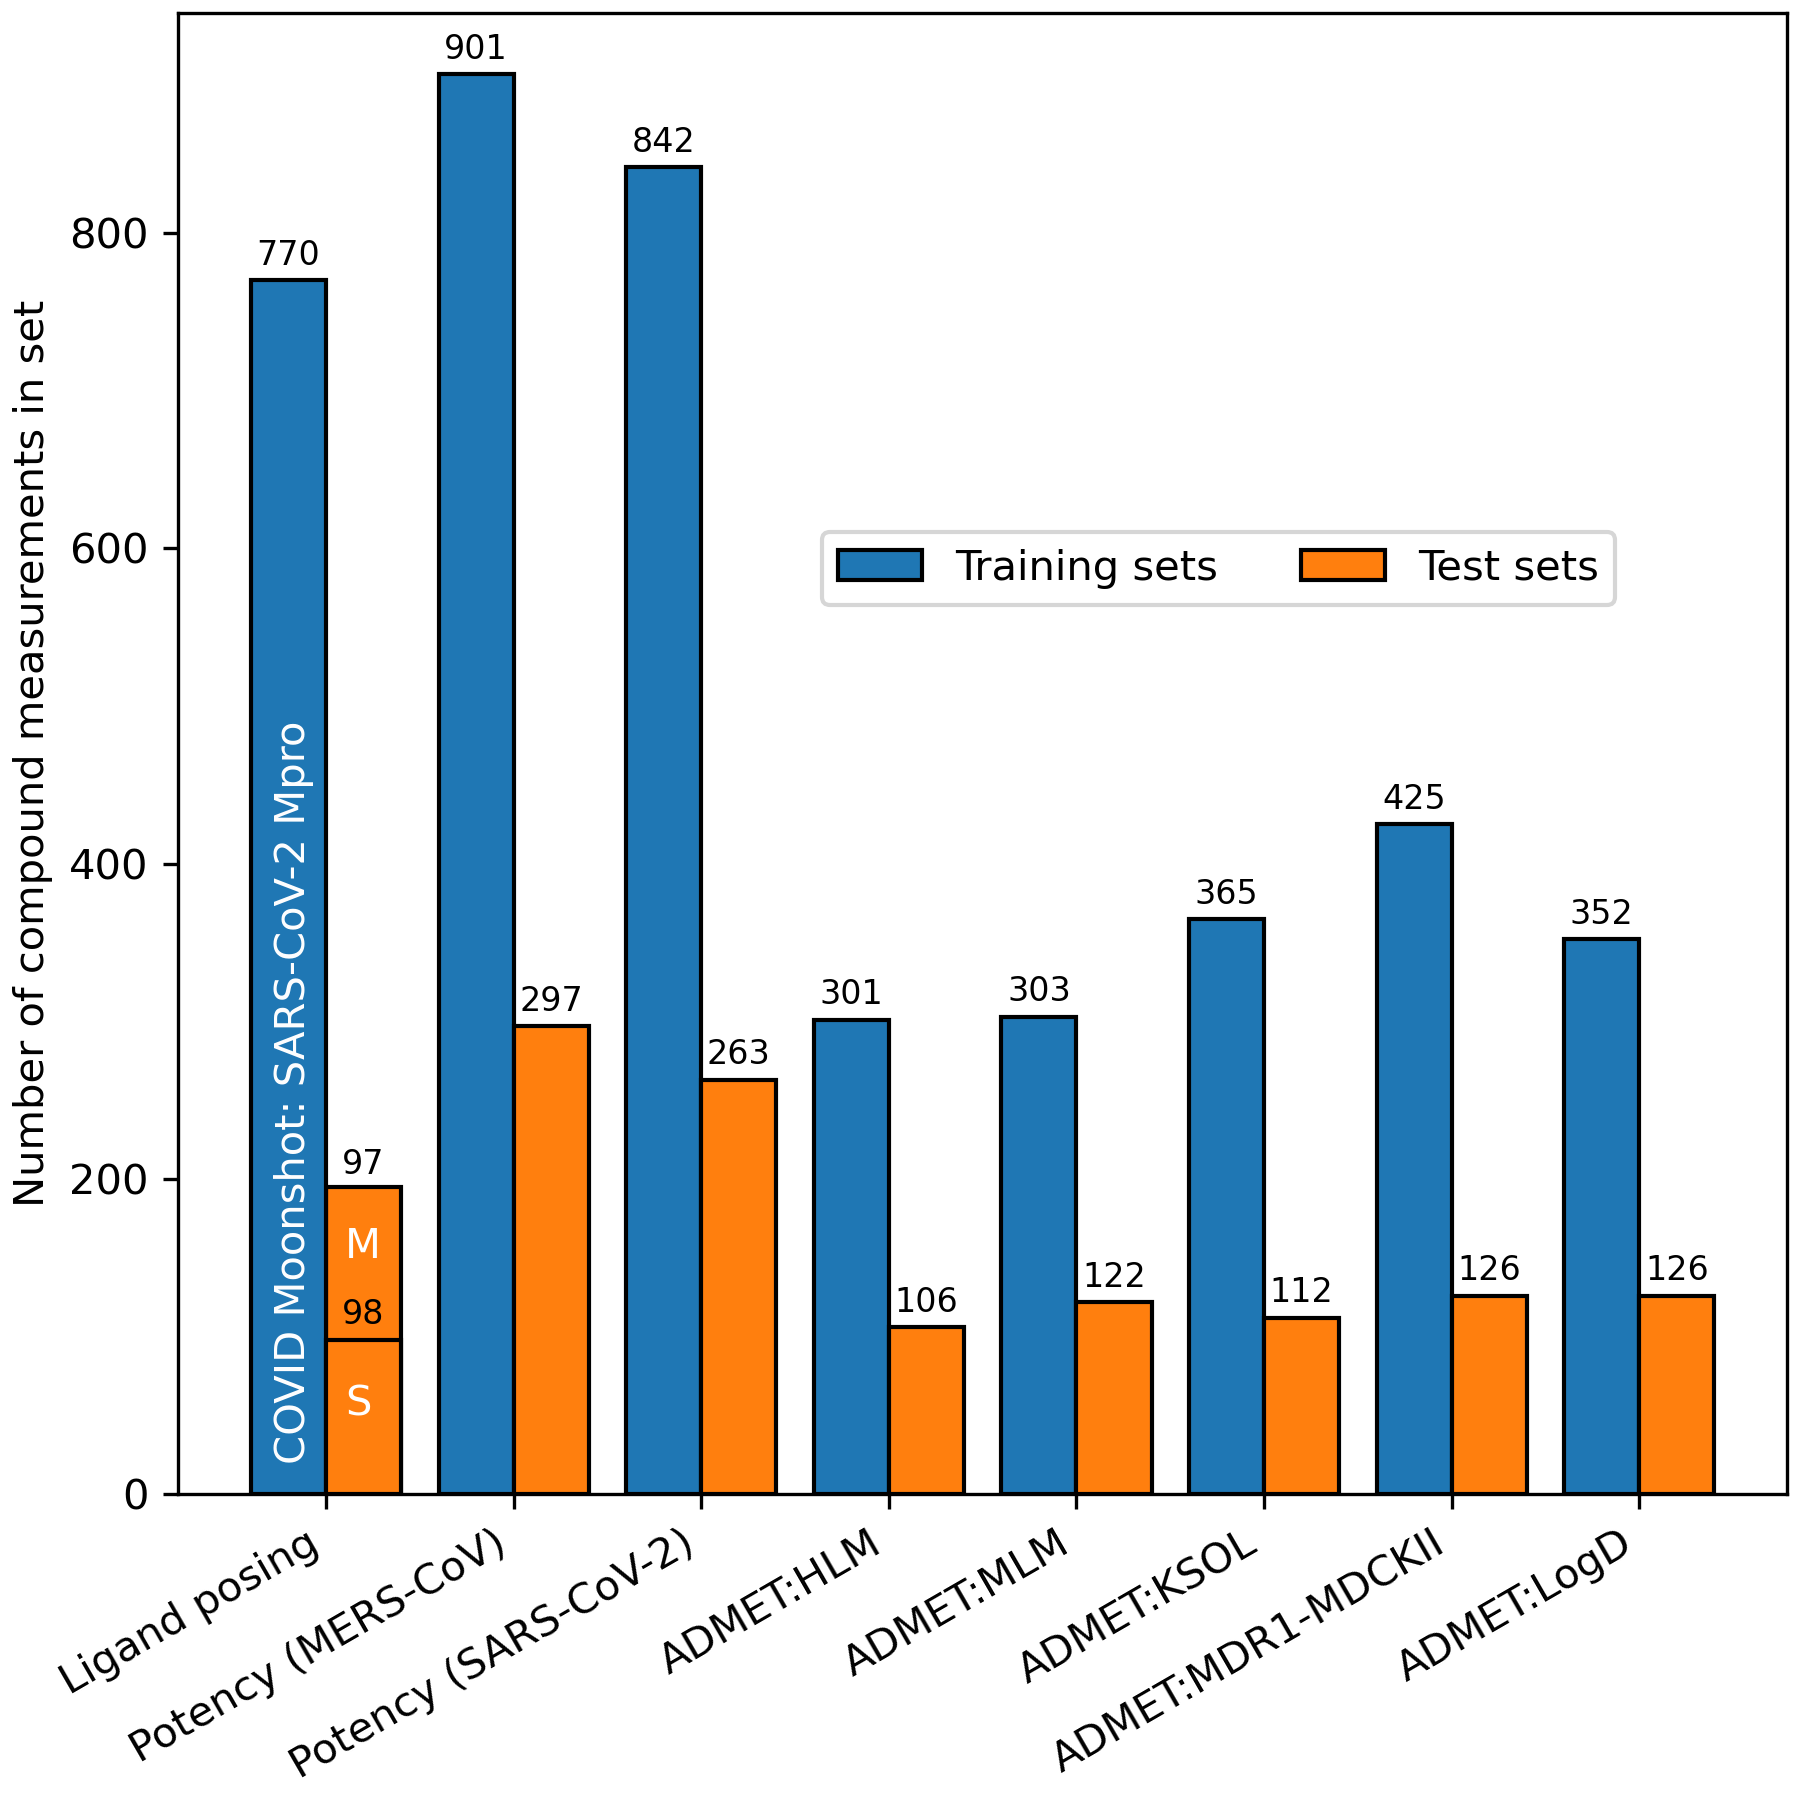
\includegraphics[scale=0.5]{01_figs_introduction/datasets_overview.png}
  \caption{Sizes of the datasets presented in this blind challenge across the different sub-challenges. Training sets are shown as blue bars and test sets as orange bars with the total number of measurements annotated at the top of each bar. For the ligand posing sub-challenge, \textbf{M} and \textbf{S} signify \textit{MERS-CoV Mpro} and \textit{SARS-CoV-2 Mpro} respectively. }
  \label{fgr:datasets_overview}
\end{figure}


%% MAIN OUTCOMES OF THE CHALLENGE

This paper aims to summarize the results of the challenge and contextualize the accompanying papers in the JCIM special issue, \textit{Open Science and Blind Data: The Antiviral Discovery Challenge}, in which participant's will describe their approaches in greater detail. Overall, the challenge saw broad engagement with a global audience, including 381 challenge submissions across 66 unique participants---with a total of 93 submissions for the final leader-board. Significant post-challenge engagement was also observed with robust scientific discussion during and after the challenge and several participating groups submitting their methods to the accompanying special issue. Robust global participation across industry and academia demonstrates ongoing interest in blind challenges, which could serve as an unbiased anchoring point to drive progress in computational methods for drug discovery in the future. 

The paper is divided as follows: we first describe the platform and overall challenge design, then detail the data collection and preparation process, including an example of how the challenge was executed in the Polaris platform, as well as describe the evaluation procedures and metrics. Finally, we discuss the main outcomes and key lessons of the challenge, providing an outlook on future implementations of similar blind challenges.

%%%%%%%%%%%%%%%%%%%%%%%%%%%%%%%%%%%%%%%%%%%%%%%%%%%%%%%%%%%%%%%%%%%%%
%% COMMUNITY
%%%%%%%%%%%%%%%%%%%%%%%%%%%%%%%%%%%%%%%%%%%%%%%%%%%%%%%%%%%%%%%%%%%%%
\section{Platform \& Community}

\subsection{Polaris provides a robust platform for benchmarking}

 Polaris provides a Python API based platform to enable easy access to drug discovery datasets and benchmarks. Serving as a single source of truth, Polaris enables access to ML-ready datasets and reproducible benchmarking. By enabling direct benchmark comparison and reducing the potential for data mishandling to influence benchmark results, modeling strategies can be assessed in a consistent way over time. Relative to similar platforms such as Kaggle, Polaris includes dedicated support for modalities common in drug discovery, including small molecules, proteins and multi-omics data and is built with best practices for these modalities in mind. Polaris' support for multiple drug discovery relevant modalities was critical for the multi-modal nature of the challenge.  Additionally, Polaris is able to leverage significant expertise from their advisory board comprised of academic and industry experts around best practices for model evaluation and benchmarking that we were able to employ in the challenge. Open, real world dataset benchmarks hosted on Polaris can help build trust in computational methods for drug discovery.

\subsection{Engaging the community}

Engaging with the scientific community and attracting high quality participants across academia and industry is critical to running an impactful blind challenge. Polaris has built significant momentum around both their platform and disseminating best practices, and have used a Discord server for community engagement. For the running of the challenge, we created a specific channel  that participants used prior, during and after the challenge for scientific and technical discussion, with the challenge responsible for significant growth in overall engagement on the Discord (Figure \ref{fgr:timeline_engagement}A). This provided a facile way for organizers to communicate with participants, as well as for participants to assist each other and discuss results. 


The challenge was designed to run in stages to maximize community engagement and allow feedback from participants. These stages were delineated by two intermediate leaderboards to enable participants to gather feedback on the performance of their modeling strategies and engage on appropriate evaluation metrics. We also conducted two office hours sessions at which participants could engage with the experimentalists that generated the challenge data and ask in-depth questions. The end of the challenge and final leaderboard was timed to coincide with the disclosure of the ASAP preclinical pan-coronavirus Mpro candidate at ACS Spring 2025\cite{griffen_2025_acs}, after which data could be freely unblinded.  The full challenge timeline can be seen in Figure \ref{fgr:timeline_engagement} B.

%\subsection*{Challenge timeline} 

%The timeline for the blind challenge is summarized in Figure \ref{fgr:timeline_engagement}B.
Additionally, as part of our public outreach campaign, we conducted extensive social media campaigns to advertise both the office hours and challenge as a whole and organized a post-challenge symposium for top-performing participants to share their methodologies (with a recording available on YouTube). 


\begin{figure}
    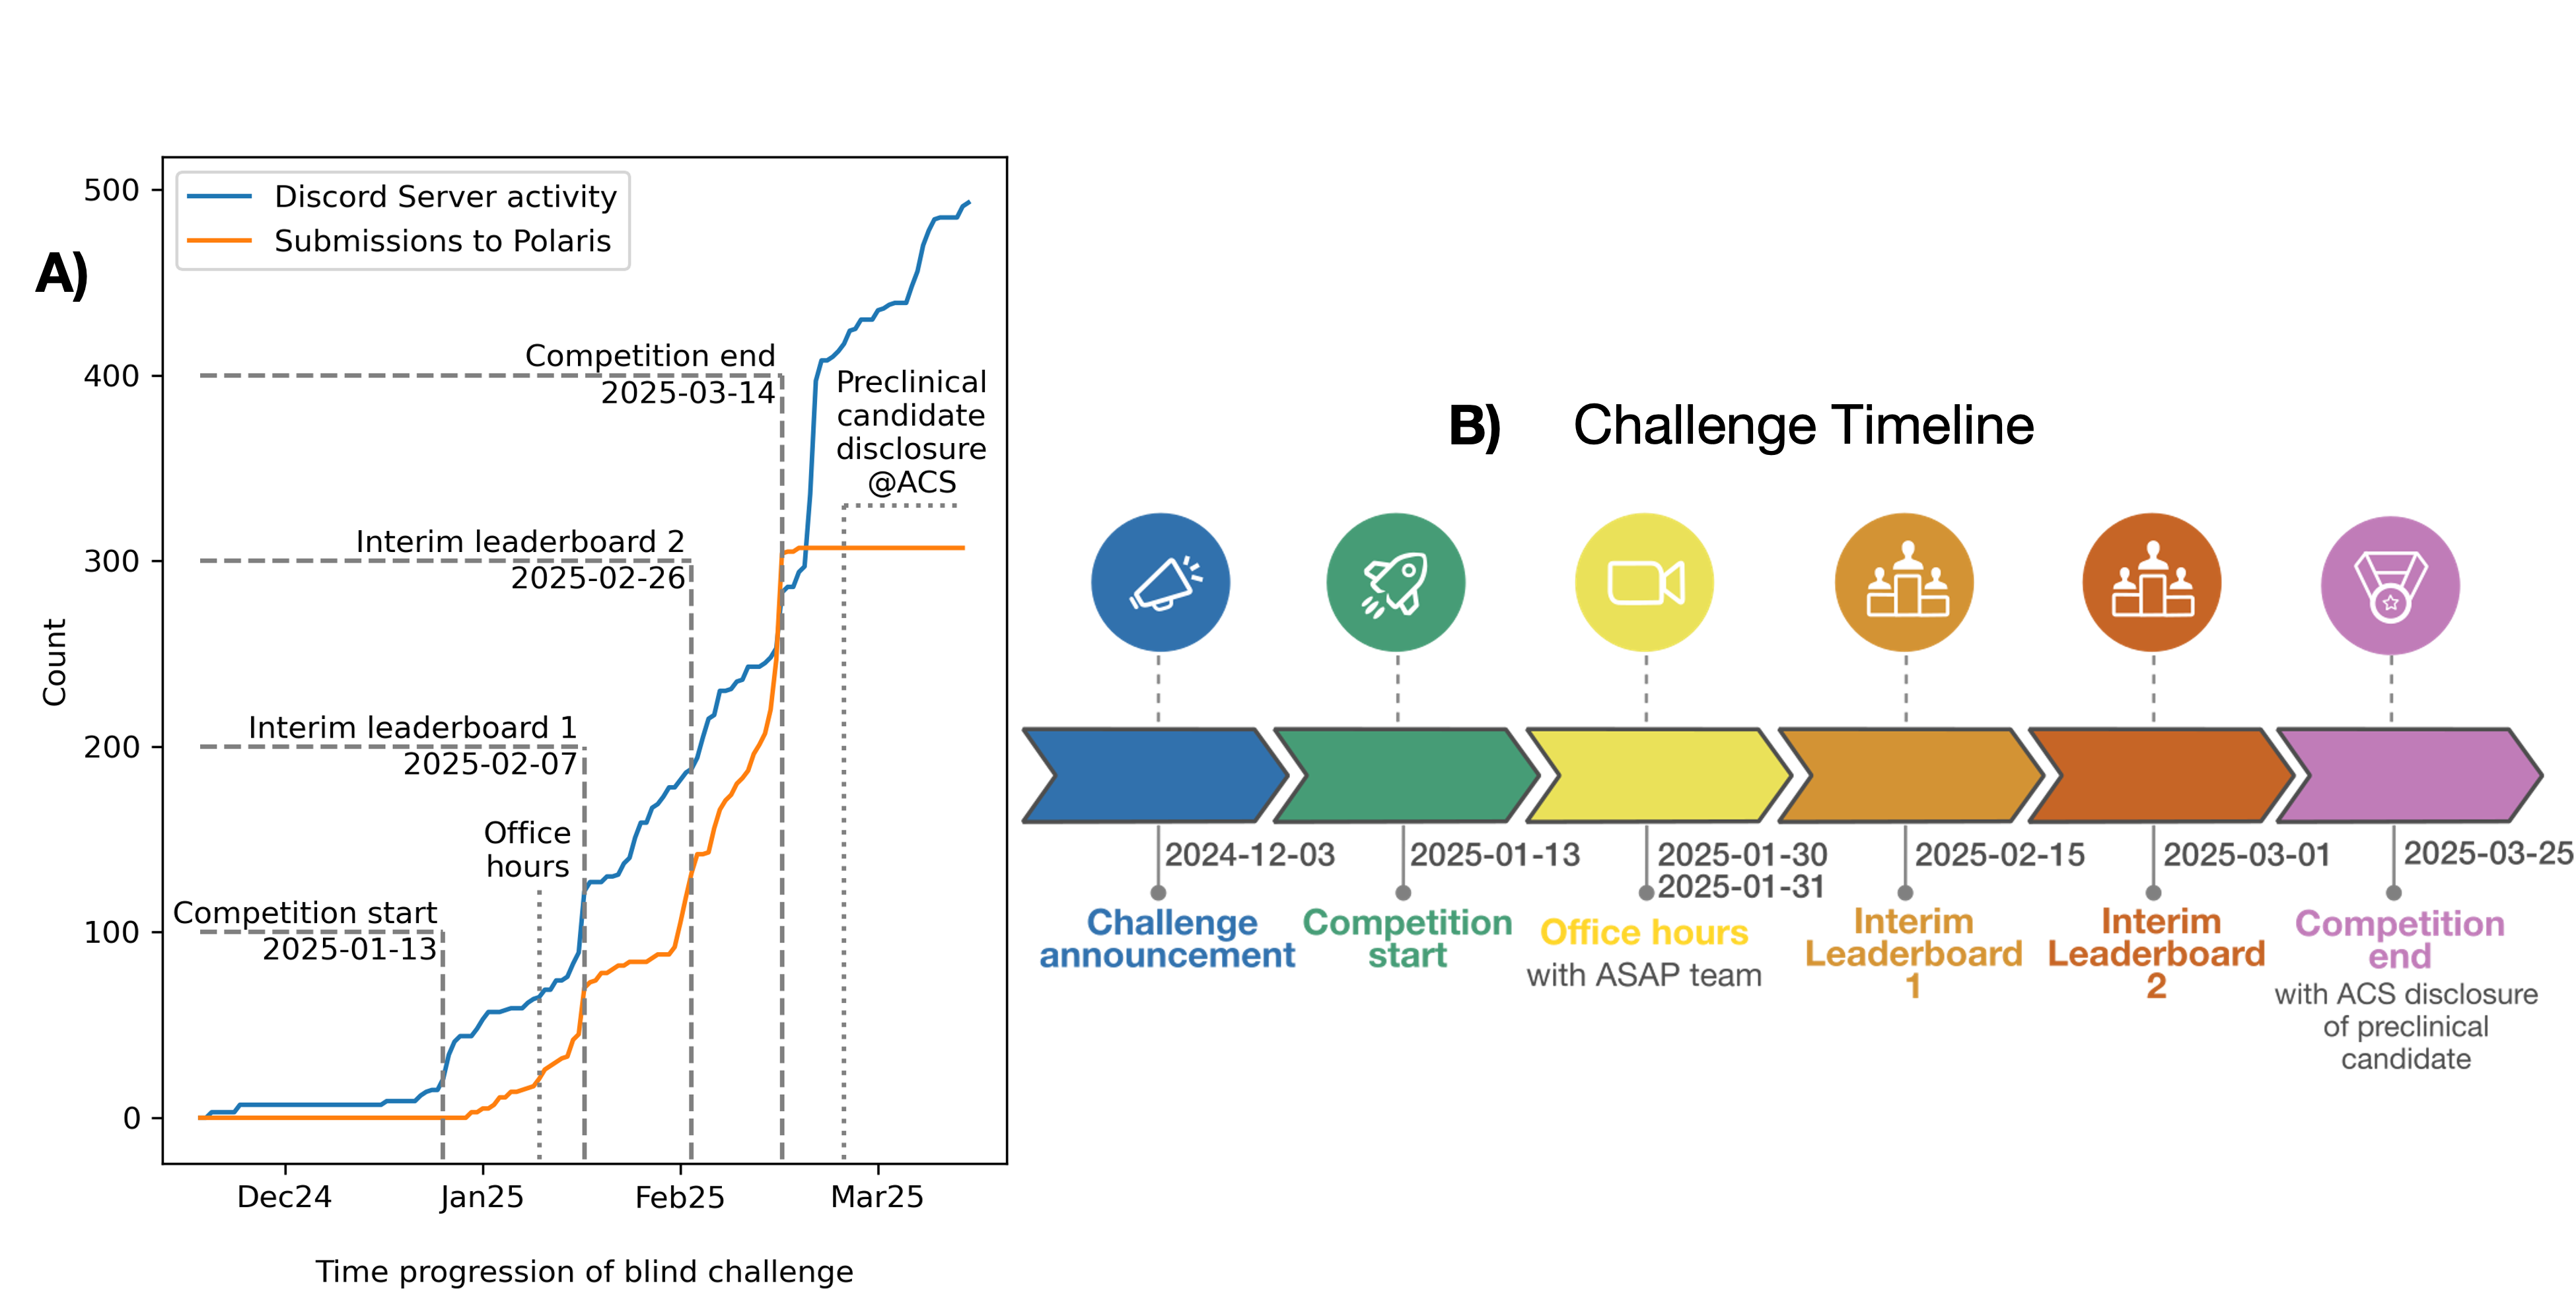
\includegraphics[scale=0.58]{02_figs_community/community_progress_and_timeline.png}
  \caption{A) Community engagement for the blind challenge across its runtime with several milestones annotated with corresponding dates. Shown are the number of messages sent by participants over the Discord server in blue and the number of predictions submitted by participants to the Polaris platform in orange. Dotted lines indicate the virtual office hours that were hosted on 2025-01-30 and 2025-01-31 and the preclinical candidate disclosure at ACS on 2025-03-25; after this date all test set data was published. B) Schematic illustration of the timeline for the ASAP-Polaris-OpenADMET Challenge, with dates annotated.}
  \label{fgr:timeline_engagement}
\end{figure}

\begin{figure}
    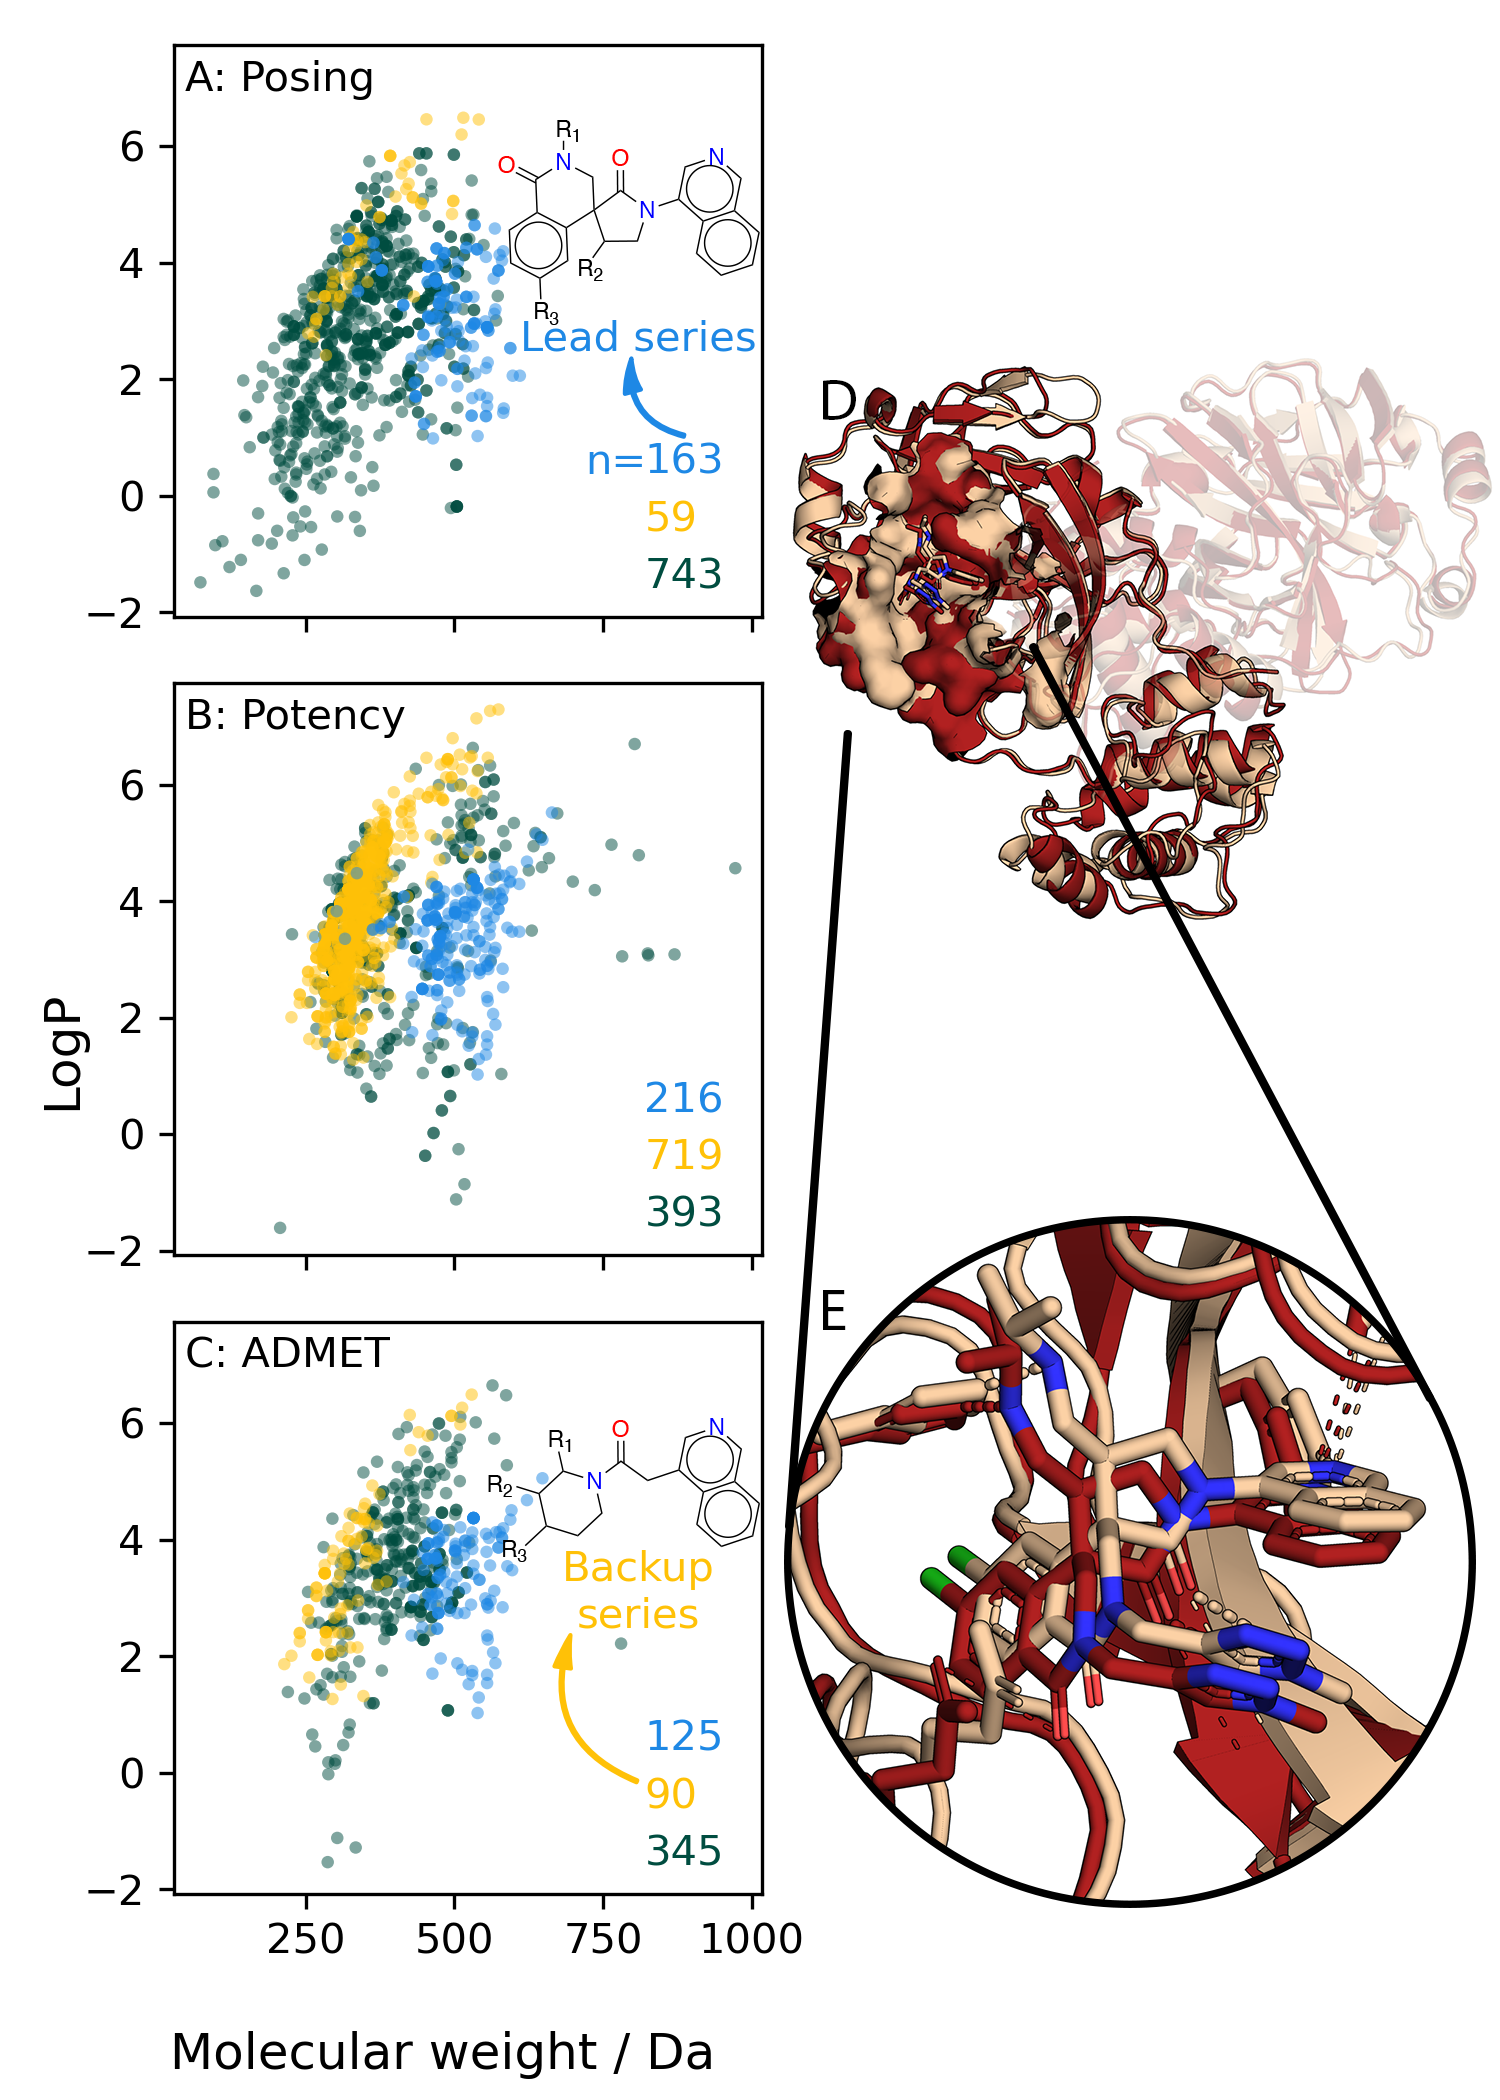
\includegraphics[scale=0.9]{03_figs_data_preparation/subchallenge_physprops_with_scaffolds.png}
  \caption{Chemical matter used in each subchallenge  spans multiple chemical series, including a lead series that progressed to nomination, and backup series. }
  \label{fgr:physprops_scaffolds}
\end{figure}

%%%%%%%%%%%%%%%%%%%%%%%%%%%%%%%%%%%%%%%%%%%%%%%%%%%%%%%%%%%%%%%%%%%%%
%% DATA PREPARATION AND EVALUATION
%%%%%%%%%%%%%%%%%%%%%%%%%%%%%%%%%%%%%%%%%%%%%%%%%%%%%%%%%%%%%%%%%%%%%
\section{Data preparation \& evaluation of models}

Data was collated from ASAP Discovery’s pan-coronavirus main-protease (Mpro) inhibitor program (spanning both SARS-CoV-2 Mpro and MERS-CoV Mpro), which at the time of challenge initiation had successfully reached preclinical candidate nomination. Available data spanned three main modalities, in-vitro biochemical potency measurements, ADMET and structural biology (X-ray crystallography) across the two protein targets. Chemical matter for the challenge spanned three main series, the nominated spirolactam containing \textit{lead} series, a \textit{backup} series, and compounds that could not be readily assigned to either series via Bemis-Murcko scaffolds\cite{bemis_murcko_1996} (Figure \ref{fgr:physprops_scaffolds}). 

As part of its pandemic preparedness mission ASAP has pursued an open-science policy in conjunction with an IP strategy designed to ensure equitable and affordable global access to any derived therapeutics. This is achieved through phased open science in the early stages of drug discovery, followed by time limited confidentiality in later stages of leadopt and “minimally defensive patenting” for candidate molecules\cite{griffen_2024}. Practical implications for the challenge were that molecules previously disclosed as part of our open-science efforts and those sufficiently congeneric to molecules claimed in a minimal patent defensive patent filed but not yet disclosed (the situation at the time of the challenge) could not be included in the challenge data.


\subsection{Reference data collection}

Mpro inhibition was measured via a direct in-vitro dose-response biochemical assay, using a fluorescent Mpro substrate. Experiments were performed primarily at the Weizmann Institute of Science. Technical differences between the assays for SARS-CoV-2 Mpro\cite{sars_mpro_dose_response_protocol} and MERS Mpro\cite{mers_mpro_dose_response_protocol} are explored in their respective protocols available online (along with many others) at the ASAP protocols.io\cite{asap_protocols_io}. Following data collection, half maximal inhibitory concentrations (IC50s) were determined by fitting to dose response curves. The fitting procedure differed between SARS-CoV-2 Mpro and MERS Mpro due to differences in binding kinetics between the two proteins, both of which are homodimeric but differ in their association constants. SARS-CoV-2 Mpro used a traditional fit to the Hill equation with a four parameter logistic function. For MERS Mpro, the weakly bound dimer can undergo ligand-induced dimerisation and an alternative curve fitting procedure used to account for the resulting low concentration activation. Challenge data used pIC50s (log10 IC50) as calculated from the raw IC50 values pooled from replicates. 

Crystal structures were expressed and purified by Centre for Medicines Discovery at the University of Oxford for SARS-CoV-2 Mpro and  MERS-CoV Mpro. Crystal constructs were created and soaked with compounds and analyzed at the X-ray beamline at Diamond Light Source according to the two protocols outlined for SARS-CoV-2 Mpro\cite{sars_mpro_crystal_protocol} and MERS-CoV Mpro respectively\cite{mers_mpro_crystal_protocol}. 

ADMET data was collected on an ADMET panel from Bienta, a bioassay contract research organisation that was configured specifically for the goals of the Mpro program as defined in ASAP’s Target Candidate Profile\cite{sars_mers_tcp} for its pan-coronavirus Mpro program. This consisted of five primary endpoints: Mouse Liver Microsomal (MLM) intrinsic clearance ($CL_{int}$) , Human Liver Microsomal (HLM) intrinsic clearance ($CL_{int}$) \cite{hlm_mlm_assay_protcol}, Kinetic Solubility (KSOL)\cite{ksol_assay_protocol}, LogD as a measure of lipophilicity\cite{logD_assay_protocol} and a cell permeability assay (Perm) in p-glycoprotein expressing Madin-Darby canine kidney cells (MDR1-MDCKII cells)\cite{perm_assay_protocol}.  For the cell permeability assay the apical to basolateral apparent permeability was used as the primary endpoint.


\begin{table}[ht]
\centering
\caption{Summary of Endpoints by sub-challenge}
\begin{tabular}{|l|l|l|}
\hline
\textbf{sub-challenge} & \textbf{Endpoint} & \textbf{Units} \\
\hline
\multirow{2}{*}{Potency} 
& SARS-CoV-2 Mpro pIC50 & unitless (log scale) \\
& MERS-CoV Mpro pIC50    & unitless (log scale) \\
\hline
\multirow{2}{*}{Ligand pose} 
& SARS-CoV-2 Mpro liganded crystal structures & NA \\
& MERS-CoV Mpro liganded crystal structures   & NA \\
\hline
\multirow{5}{*}{ADMET} 
& Mouse Liver Microsomal $CL_{int}$ (MLM)  & uL/min/mg \\
& Human Liver Microsomal $CL_{int}$ (HLM)  & uL/min/mg \\
& Kinetic Solubility (KSOL)               & µM \\
& LogD                                    & unitless (log scale) \\
& Cell permeability (apical-to-basolateral, MDR1-MDCKII cells) & 10\textsuperscript{-6} cm/s \\
\hline
\end{tabular}
\end{table}

\subsection{ML-ready dataset preparation}

Data was collated from ASAP’s CDD vault, a research informatics database platform that aggregates assay outcomes by molecule. Data was split into a training set that was released to participants and a blind test set that participants were evaluated on. A target 75:25 train:test split was selected for the ADMET and potency prediction challenges, while for the pose prediction challenge data from the COVID Moonshot\cite{boby_2023} (also solved by X-ray crystallography at Diamond Light Source) was used as the training set totaling 770 structures for SARS-CoV-2 Mpro only, while the test set comprised 98 SARS-CoV-2 Mpro structures and 97 MERS-CoV Mpro structures from the ASAP Discovery Consortium.  

For the ADMET and potency sub-challenges we used a temporal split of the data to create a challenge more representative of real-world drug discovery, where molecules must be evaluated prospectively\cite{sheridan_time-split_2013}. However, this had to be balanced against minimization of leakage between endpoints which could jeopardize competition integrity by revealing test set molecules to participants in the training set of other endpoints. This was particularly challenging for the ADMET sub-challenge in which several endpoints have limited amounts of data, meaning that a multi-endpoint, multi-sub-challenge split had to be carefully designed to minimize leakage between endpoints and sub-challenges. 

To balance these competing concerns, the following hybrid splitting procedure was followed for the ADMET and potency sub-challenges. First, all molecules in common between both the ADMET and potency sub-challenge were determined (N=197 in raw data package). The split for each endpoint that minimizes leakage across all endpoints and datasets will contain as many of the shared molecules as possible in the \textbf{test set} such that the test set can "hold out" as many structures as possible across the totality of compounds. For the potency sub-challenge, this was achieved by first placing the common molecules in the test set and then adding remaining molecules newest-first by MERS Mpro potency assay date to the test such such that the test set is biased towards newer compounds (simulated time based split). This split (common augmented with MERS Mpro date-ordered) was then used to also split the SARS-CoV-2 data.   MERS Mpro potency assay date was chosen to bias the time based element of the split as generally speaking MERS Mpro assays were enabled after SARS-CoV-2 Mpro assays, providing a better bias towards newer compounds. Note that in this splitting procedure, tradeoff between leakage and split ratios results in the elimination of leakage \textit{within the potency challenge} but with some variation in the exact 75:25 train-test split ratio by endpoint (SARS-CoV-2 Mpro pIC50 vs MERS Mpro pIC50). Overall this procedure can be thought of as a leakage minimizing date-biased split for a single endpoint (e.g MERS-CoV Mpro pIC50) with the other endpoint(s) split using the same indices.

For the ADMET sub-challenge a similar procedure was followed, however the number of common molecules that would need to be placed in the test set exceeds the 75:25 train-test ratio for some endpoints (Figure \ref{fgr:datasets_overview}). To minimize the impact of this while still biasing by date, the common molecules were ordered by LogD assay date and molecules selected to satisfy a 75:25 train test split. The LogD time-based split was used to also split the other endpoints such that a consistent split was shared by the ADMET endpoints, eliminating between-endpoint leakage \textit{within the ADMET sub-challenge} and biasing by date while also maximising the number of common molecules held out between the potency and ADMET sets. Given the dataset sizes and extent of overlap there is an unavoidable ~70 compounds leak between the ADMET training set and potency test set (common molecules that were not be placed in the ADMET test set). However this between-endpoint leakage is not expected to provide significant information gain to the participants given that the leaked subset cannot be known \textit{a-priori}.

Following splitting, the data was cleaned to be ML-ready. Compounds marked as below or above assay detectable range with a ChEMBL style modifier ( $<$, $<=$, $>=$, $>$) were removed. Duplicate molecules were removed, with some missed on an an initial pass and removed following detection on by participants. Where a molecule had data recorded for an endpoint more than once, the most recent data collection was selected. The final ML-ready datasets for ADMET and potency were organized as a multi-task matrix and uploaded to the Polaris platform. Datasets with out of range datapoints and some additional endpoint-specific assay data was made available for the participants in case they wanted to leverage the additional negative data in their models. The final ML-ready datasets were uploaded to the Polaris platform, with each sub-challenge represented as a multitask matrix where appropriate. See Figure \ref{fgr:datasets_overview} for an overview of the datasets available. 


\subsection{Running the challenge on the Polaris platform}

Participants uploaded their predictions to the Polaris platform via the API. Example Python code detailing how participants were expected to submit their predictions is shown in Listing \ref{code:submission}. This provides significant operational advantages relative to modes of running other challenges, which include large amounts of manual data handling. A consistent pythonic API also allows participants to co-locate their modeling efforts with submission to the challenge infrastructure e.g in a Jupyter notebook.

\begin{code}
\setminted{baselinestretch=0.5} % decreases vertical spacing between lines
\captionof{listing}{Example Python code to submit to Polaris API}
\label{code:submission}
\begin{minted}{python}
import polaris as po

# load the competition data from the Polaris platform and split it
competition = po.load_competition("asap-discovery/antiviral-potency-2025")
train, test = competition.get_train_test_split()

# make predictions
y_pred = my_participant_model(test)

# submit predictions to the Polaris platform
competition.submit_predictions(
    predictions=y_pred,
    prediction_name="my-predictions",
    prediction_owner="participant_name",
    report_url="https://www.my_report.com",
)
\end{minted}
\end{code}


To enable participants to easily use the Polaris challenge infrastructure, we provided participants example notebooks with baselines to demonstrate how to submit to each of the sub-challenges. These were made available on GitHub at the following location: https://github.com/asapdiscovery/asap-polaris-blind-challenge-examples. 

While evaluation of tabular data submissions for the potency and ADMET subchallenges did not provide technical challenges, the ligand pose subchallenge proved to be more complex. Due to technical constraints, we could not store and evaluate submissions of full protein-ligand structures for each molecule for each participant. Instead the particpants were required to submit a serialized RDKit molecule of the ligand only, pre-aligned to a reference structure. While circumventing technical issues, this solution did rely on participants correctly aligning their results with the reference structure, which proved challenging for some submissions (see Challenge Outcomes).


Participants were required to submit prior to the final leaderboard cutoff date with only their last submission counting towards the leaderboard. Additionally to be eligible for the final leaderboard participants were required to provide either a link to code detailing their methods, or a short written report. This done was to ensure that shared learnings could be derived from ranking of the modeling approaches while still allowing participants (particularly those in industry) to preserve proprietary code. 

Following the conclusion of the challenge, we also open-sourced the challenge data as presented to the participants on the Polaris platform, allowing continued engagement with the challenge consistent with the way in which it was originally run. 


\subsection{Evaluation procedure}    

Fair and robust prediction evaluation is critical to the success of a blind challenge. Evaluation of computational predictions for chemical matter in drug discovery is evolving, with several recent papers outlining best practices in this area.  Robust evaluation is critical for building trust and to the adoption of \textit{ in silico} methods. With this in mind, we developed a rigorous evaluation procedure that would fairly evaluate participants' submissions while remaining easily interpretable to outside participants.

Evaluation procedures and metrics were chosen for each sub-challenge based on the data distributions and appropriate treatment for the data modality. For each sub-challenge, multiple metrics were reported, with one metric chosen for primary ranking. Where a sub-challenge was comprised of multiple endpoints (SARS-CoV-2 Mpro pIC50 and MERS-CoV Mpro pIC50 for potency, MLM, HLM, KSOL, LogD and Perm for ADMET) the macro-averaged primary metric was used for ranking. For the potency and ADMET sub-challenges the Mean Absolute Error (MAE), Mean Squared Error (MSE), Pearson's $R$, Spearman's $\rho$ and $R^2$ were reported. For the ligand pose sub-challenge, the success rate (number of poses with a ligand heavy atom RMSD below a threshold) at a threshold of 2Å was reported.

For the potency sub-challenge, MAE was chosen as an appropriate flexible continuous metric for potency evaluation. Ranking of compounds by potency is often viewed as at least as important as absolute potency prediction. To this end we also conducted analyses of Kendall's Tau, assessing the ability of participants to rank-order potent molecules. 

For the ADMET sub-challenge, MAE was chosen as the primary metric. Values for ADMET endpoints span a wide range with significant outliers. To alleviate the impact of outliers on the evaluation, endpoints that were not already in a base 10 logarithmic scale (LogD) were transformed to a base 10 logarithmic scale prior to evaluation with metrics (MAE, MSE, Pearson's $R$, Spearman's $\rho$ and $R^2$). As some endpoints had values at exactly 0, a $ y=log_{10}(x + 1)$ transform was used. Overall the effect of this transformation was to log-normalize the endpoints prior to evaluation and minimize the impact of outliers on evaluation metrics (see SI Figure \ref{fgr:admet_endpoints}).  

To robustly assess relative model performance, statistical hypothesis based comparison is required. Due to stochasticity inherent in computational modeling ideally a population of models would be prepared for each submission via techniques such as cross validation and variation in model performance assessed via comparison of distributions of metrics. As this was judged to be too challenging for every participants to adhere to, populations of metrics were instead computed via bootstrapping. While this likely underestimates the variance in metric populations, this approach allows calculation of estimated confidence intervals without large technical overhead. Following calculation of metric populations via bootstrapping, models were compared pairwise using Tukey's Honestly Significant Difference (HSD) test in accordance with a recent whitepaper detailing best practices for model comparison. Leaderboard rankings results and associated statistical difference testing between models was communicated using Compact Letter Display (CLD), where models are ordered alphabetically by performance, where models sharing a letter are not statistically distinct. 


Importantly evaluation logic was open-sourced on GitHub at the following location: https://github.com/asapdiscovery/asap-polaris-blind-challenge-examples, allowing participants to engage with the evaluation procedures and metrics. The evaluation logic was revised several times following feedback from participants including the exclusion of some duplicates that were missed in the initial preparation logic, and some racemic compound measurements that differed only in their extended stereochemistry (e.g 'and' or 'or' stereochemistry). Additionally some the ligand pose subchallenge required some additional pooling logic to deal with compounds for which more than one X-ray structure was available (e.g in different space groups). 


We also provided baselines for each of the challenge modalities, meant to represent minimal effort approaches to modeling each respective endpoint and provided useful calibration for more complex approaches. For the potency sub-challenge, a linear model based of ECFP fingerprints was used, as trained on the training set. For the ADMET challenge a linear model of cLogP was used for each endpoint as trained on the training set. For the poses sub-challenge, two baselines were prepared. A performance baseline similar to standard docking procedure was at ASAP was used, with cross-docking of each input molecule on the 5 closest available structures (ranked by RascalMCES) conducted using OpenEye POSIT and the highest scoring pose by ChemGauss4 score selected. A "blind docking" baseline was also prepared using GNINA, with the docking box placed in the known Mpro binding site. Full code to run the baselines is available on GitHub at the following location: https://github.com/asapdiscovery/asap-polaris-challenge-baselines. 

%%%%%%%%%%%%%%%%%%%%%%%%%%%%%%%%%%%%%%%%%%%%%%%%%%%%%%%%%%%%%%%%%%%%%
%% OUTCOMES
%%%%%%%%%%%%%%%%%%%%%%%%%%%%%%%%%%%%%%%%%%%%%%%%%%%%%%%%%%%%%%%%%%%%%
\section{Challenge Outcomes}

Outcomes across the subchallenges were evaluated through analysis of final leaderboards and distributions of model performance on each subchallenge and its associated endpoints. Where models are categorized, (e.g deep learning, traditional ML, cofolding, physics based) we have collected this information from the reports or code mandated for the final leaderboard (see Table \ref{tbl:categories} for a full breakdown). Possible impact of models with respect to ASAP's leadopt goals as stated in the TCP\cite{sars_mers_tcp} are also explored. 

\subsection{Potency}


\begin{figure}
    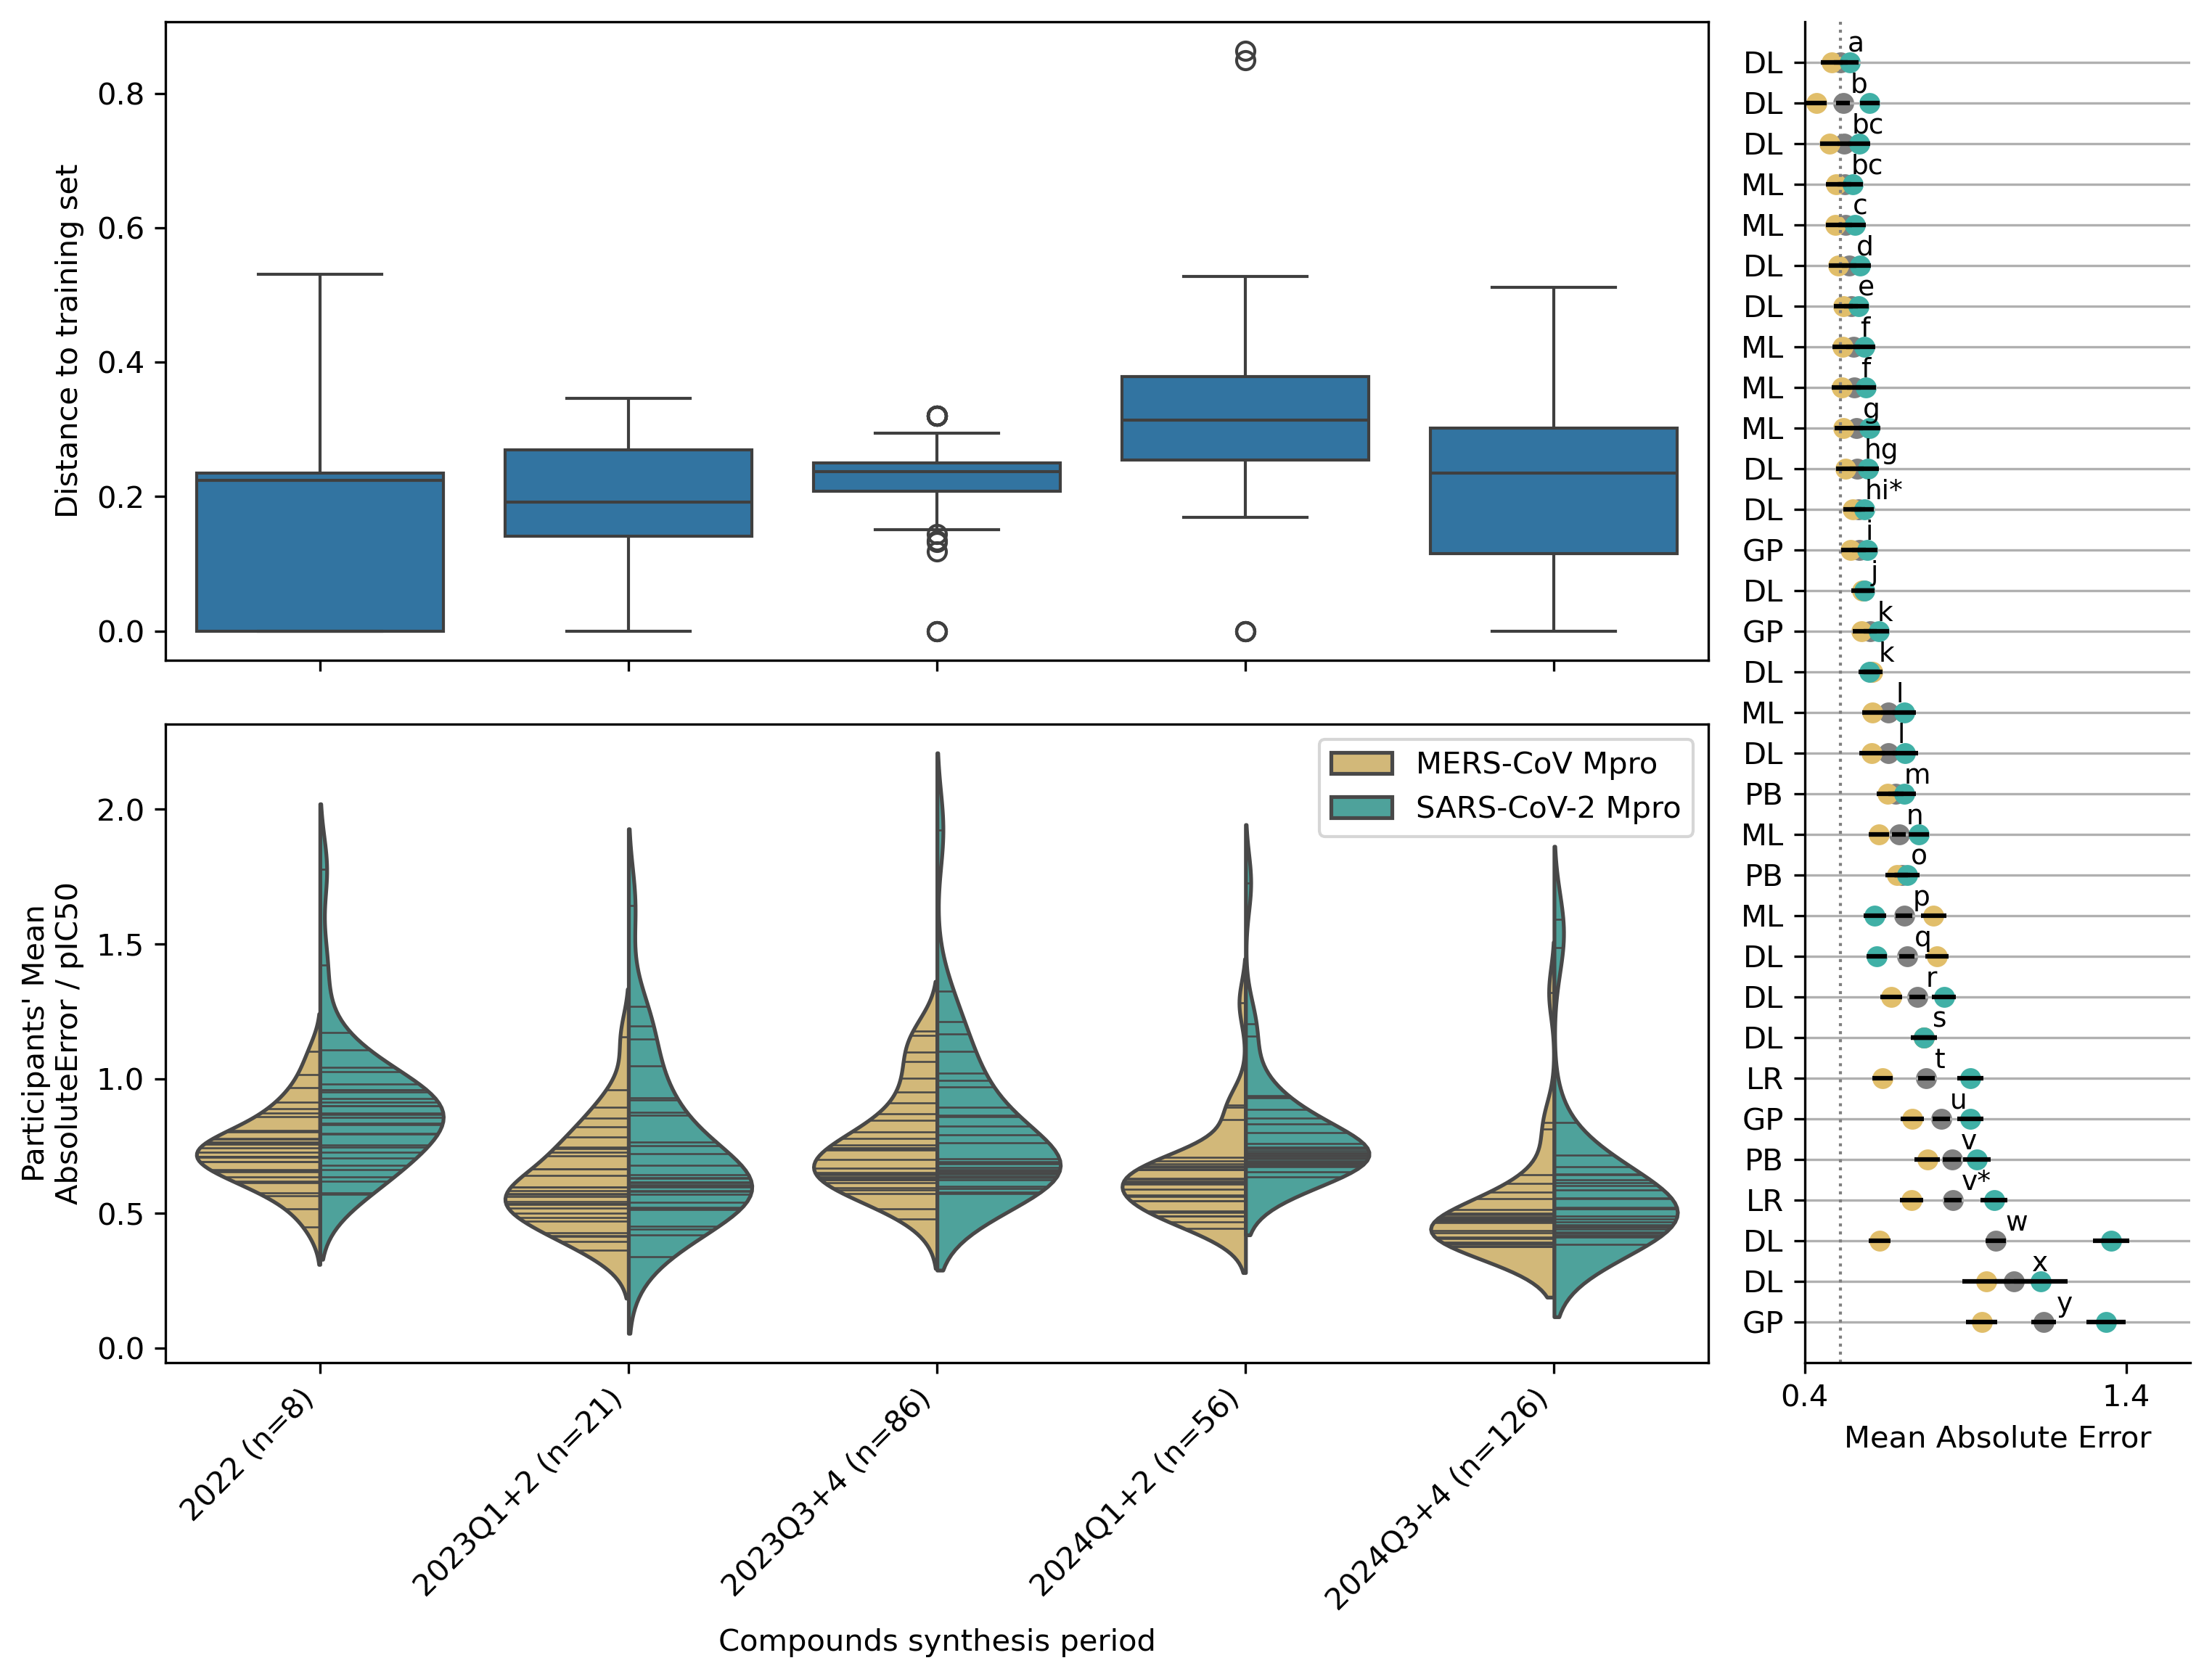
\includegraphics[scale=0.6]{04_figs_leaderboards/potency_leaderboards_and_progressions.png}
  \caption{Participants performed diversely on potency predictions. A) the Jaccard fingerprint distance to the training set of compounds in the test set split by the period the compound was actioned for synthesis. B) participants' performance on each collection of compounds (as split in A) in mean absolute error of pIC50. An additional split by target (MERS-CoV Mpro in yellow, SARS-CoV-2 Mpro in green) is shown. C) leaderboard of the potency subchallenge as each entry's category (DL=Deep Learning, ML=Machine Learning, PB=Physics-Based, GP=Gaussian Process, LR=Linear Regression) and split by target in the same colors as B). Baseline models as deployed by the organisers are marked with asterisks. Each entry is annotated with its statistical ranking by the Compact Letter Display (CLD) system.}
  \label{fgr:potency_leaderboards}
\end{figure}

% General description of performance %
Participants performance in the potency prediction subchallenge varied by methodology with deep learning and machine learning models outperforming physics based and other approached across the board \ref{fgr:potency_leaderboards}. Top performing entries performed well across both MERS-CoV and SARS-CoV-2 Mpro binding, with top models generally performing slightly better for the MERS-CoV endpoint relative to SARS-CoV-2. Examination of participants performance (MAE) relative to ECFP Tanimoto distances to the training set indicated that chemical similarity to the training set did not meaningfully assist model predictions across the test set. A time-wise breakdown of the test set by synthesis date also revealed limited influence of synthesis date on model performance. While general trends surrounding similarity to the training set and synthesis date could not be established, it is possible the noise from less performant models obstructs trends seen in more performant models.


% How well do people do in real terms %
Top performing participants were able to predict potency with a high degree of accuracy (macro-average MAE of 0.509 ± 0.022 (a)
, 0.516 ± 0.022 (b), 0.517 ± 0.021 (bc) for the top three entries respectively). Top performing methodologies outperformed existing graph attentional neural networks employed at ASAP to predict affinities (12th best entry, CLD: \textit{h1*}), and would have likely greatly assisted compound prioritization within our leadopt campaign. Most participants were able to outperform the ECFP linear regression baseline (29th entry, CLD: \textit{v*}) Participants ability to rank compounds by potency was also generally strong, with the top three performing entries displaying Kendall's Tau's of 0.626 ± 0.016, 0.649 ± 0.018 and 0.614 ± 0.018 respectively. As with the ability of these top performing models to predict absolute pIC50s to within approximately half a log unit, their ability to rank compounds by affinity was also impressive, considering that typical experimental potency measurement assays are expected to have an intrinsic variance of 0.2-0.4 log units.

% How did they do it %
Analysis of top performing affinity prediction methods reveals a diverse set of deep learning approaches including the MolE and MolGPS graph neural network (GNN) foundation models. Other performant approaches included using pre-computed features from representation learning models combined either with traditional ML models (e.g SVMs) or further neural network layers. Many participants also employed ensembling to improve model performance.  Importantly many of the top performing models (including all of the top 3) employed some kind of pre-training step involving large numbers of unlabeled chemical structures outside of the challenge data to develop embeddings for downstream task prediction.


\subsection{ADMET}

In order to compare across ADMET endpoints the endpoint MAE was normalized to the dynamic range for each endpoint (here referred to as the relative absolute error, RAE). As with the potency subchallenge model's ability to rank order compounds in the ADMET subchallenge was assessed using Kendall's Tau. Participants performance varied across the endpoints with the solubility (KSOL) and LogD endpoints appearing the easiest to predict in relative terms. However when ranking ability is examined, the inability of even the best performing models to rank compounds by solubility is revealed, contrasting the excellent ranking performance of LogD models \ref{fgr:admet_endpoints}.  Poor performance on solubility ranking is attributable both to the dynamic range available in the training set (most compounds fall generally into the range considered soluble) and also the noted difficulty of predicting solubility prospectively across several benchmarks. Given good RAE performance and poor ranking ability for the KSOL endpoint, it is likely that models are memorizing the absolute solubility of the training set, performing closer in practice to a classification model. This is not necessarily an issue as in practice solubility is considered a quasi-classification problem where compounds are handled as being either soluble or insoluble by scientists. HLM and MLM performance was similar across challenge entries with these proving to be the hardest to predict in relative (RAE) terms. Ranking performance across HLM and MLM was generally strong with top performing models achieving Kendall's Tau's between 0.5 and 0.6, As with potency, generally the best performing models overall were performant across all endpoints.

% How well do people do in real terms %
Top perfoming models XXXXX.


% How did they do it %
Analysis of XXXX


\begin{figure}
    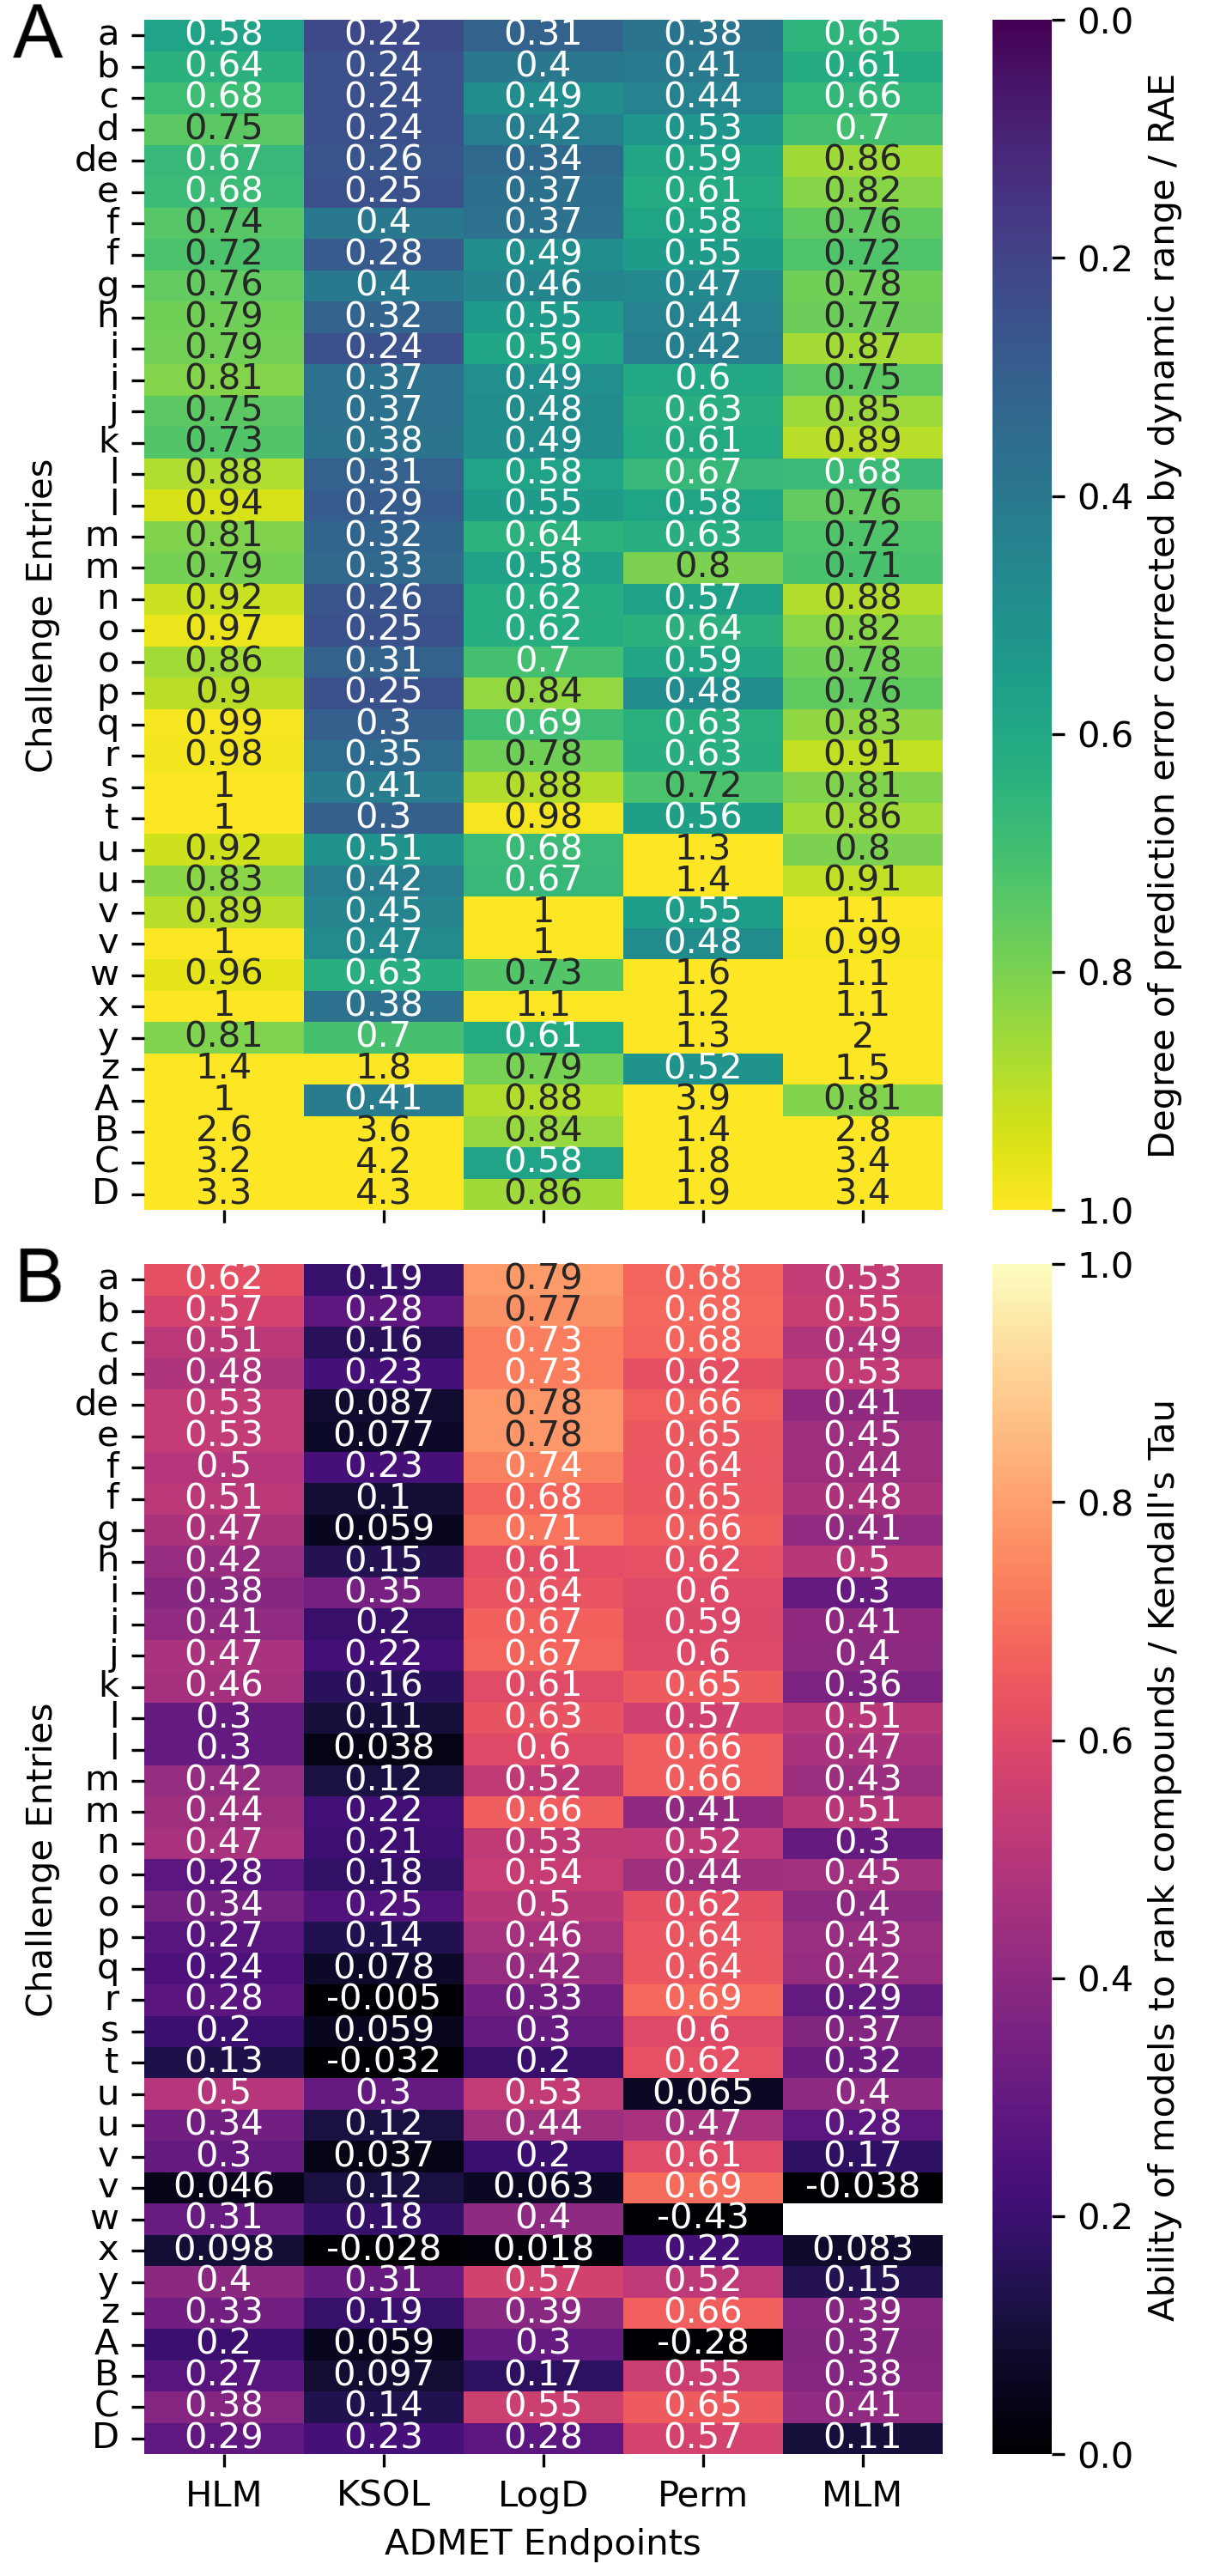
\includegraphics[scale=0.6]{04_figs_leaderboards/heatmaps.png}
  \caption{Participants' models performed poorly on kinetic solubility predictions but strongly on stability, permeability and lipophilicity. Shown are (A) the relative absolute error of the normalized, predicted challenge endpoints, and (B) the Kendall's Tau of the normalized, predicted challenge endpoints. The empty cell at entry \textit{w} MLM consisted of constant predicted values thus no ranking coefficient was calculated. Entries are ranked by their macro-averaged MAE over all endpoints}
  \label{fgr:heatmaps_admet}
\end{figure}

\subsection{Ligand Poses}

\begin{figure}
    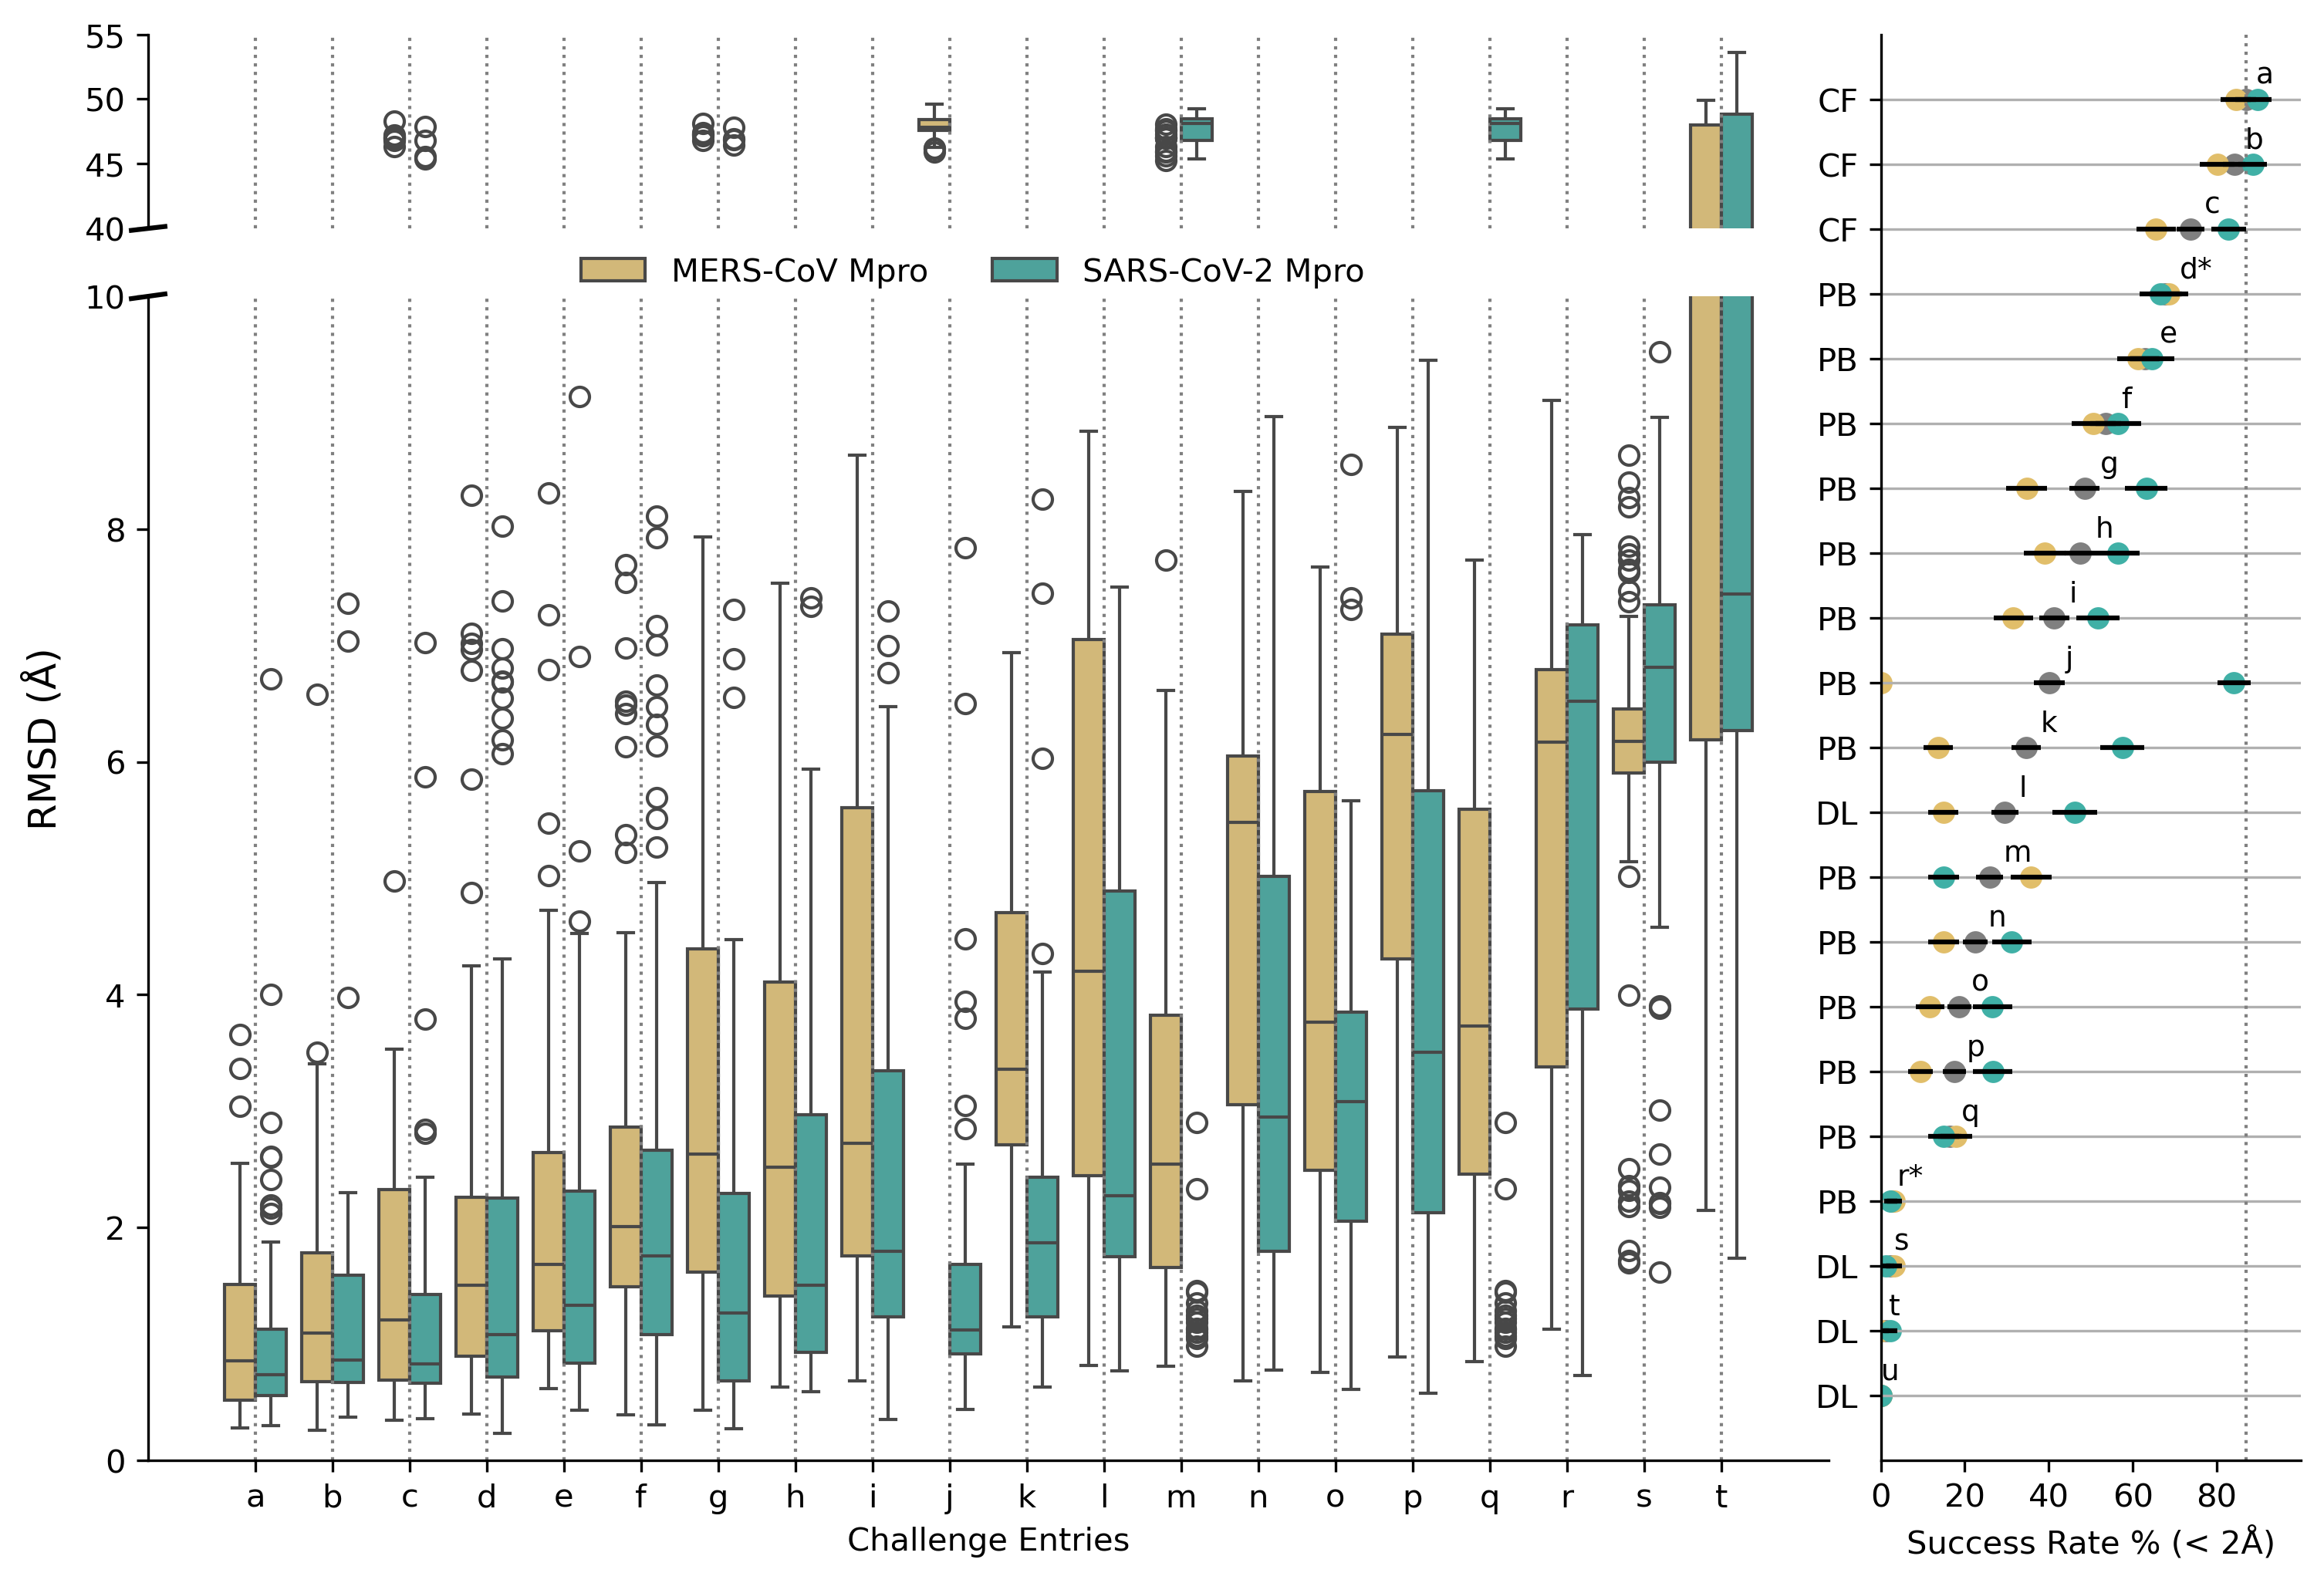
\includegraphics[scale=0.15
    ]{04_figs_leaderboards/pose_comp.png}
  \caption{Participants' generally performed better on the SARS-CoV-2 pose predictions with higher success rates, ligands predicted with an RMSD \textless2Å, and lower median RMSD predictions apart from one entry, \textit{m,} which shows the reverse prediction accuracy. Prediction RMSD distributions are shown for each entry split by the MERS-CoV and SARS-CoV-2 Mpro targets (left) with one entry removed u as the full distribution lies in the axis break. The success rate of each entry is shown (right) for the overall submission (grey) and the two targets separately to further highlight the difference in performance across the targets. The overall success rate was used to determine the final ranking of the submissions.}
  \label{fgr:poses_leaderboard}
\end{figure}


\begin{figure}
    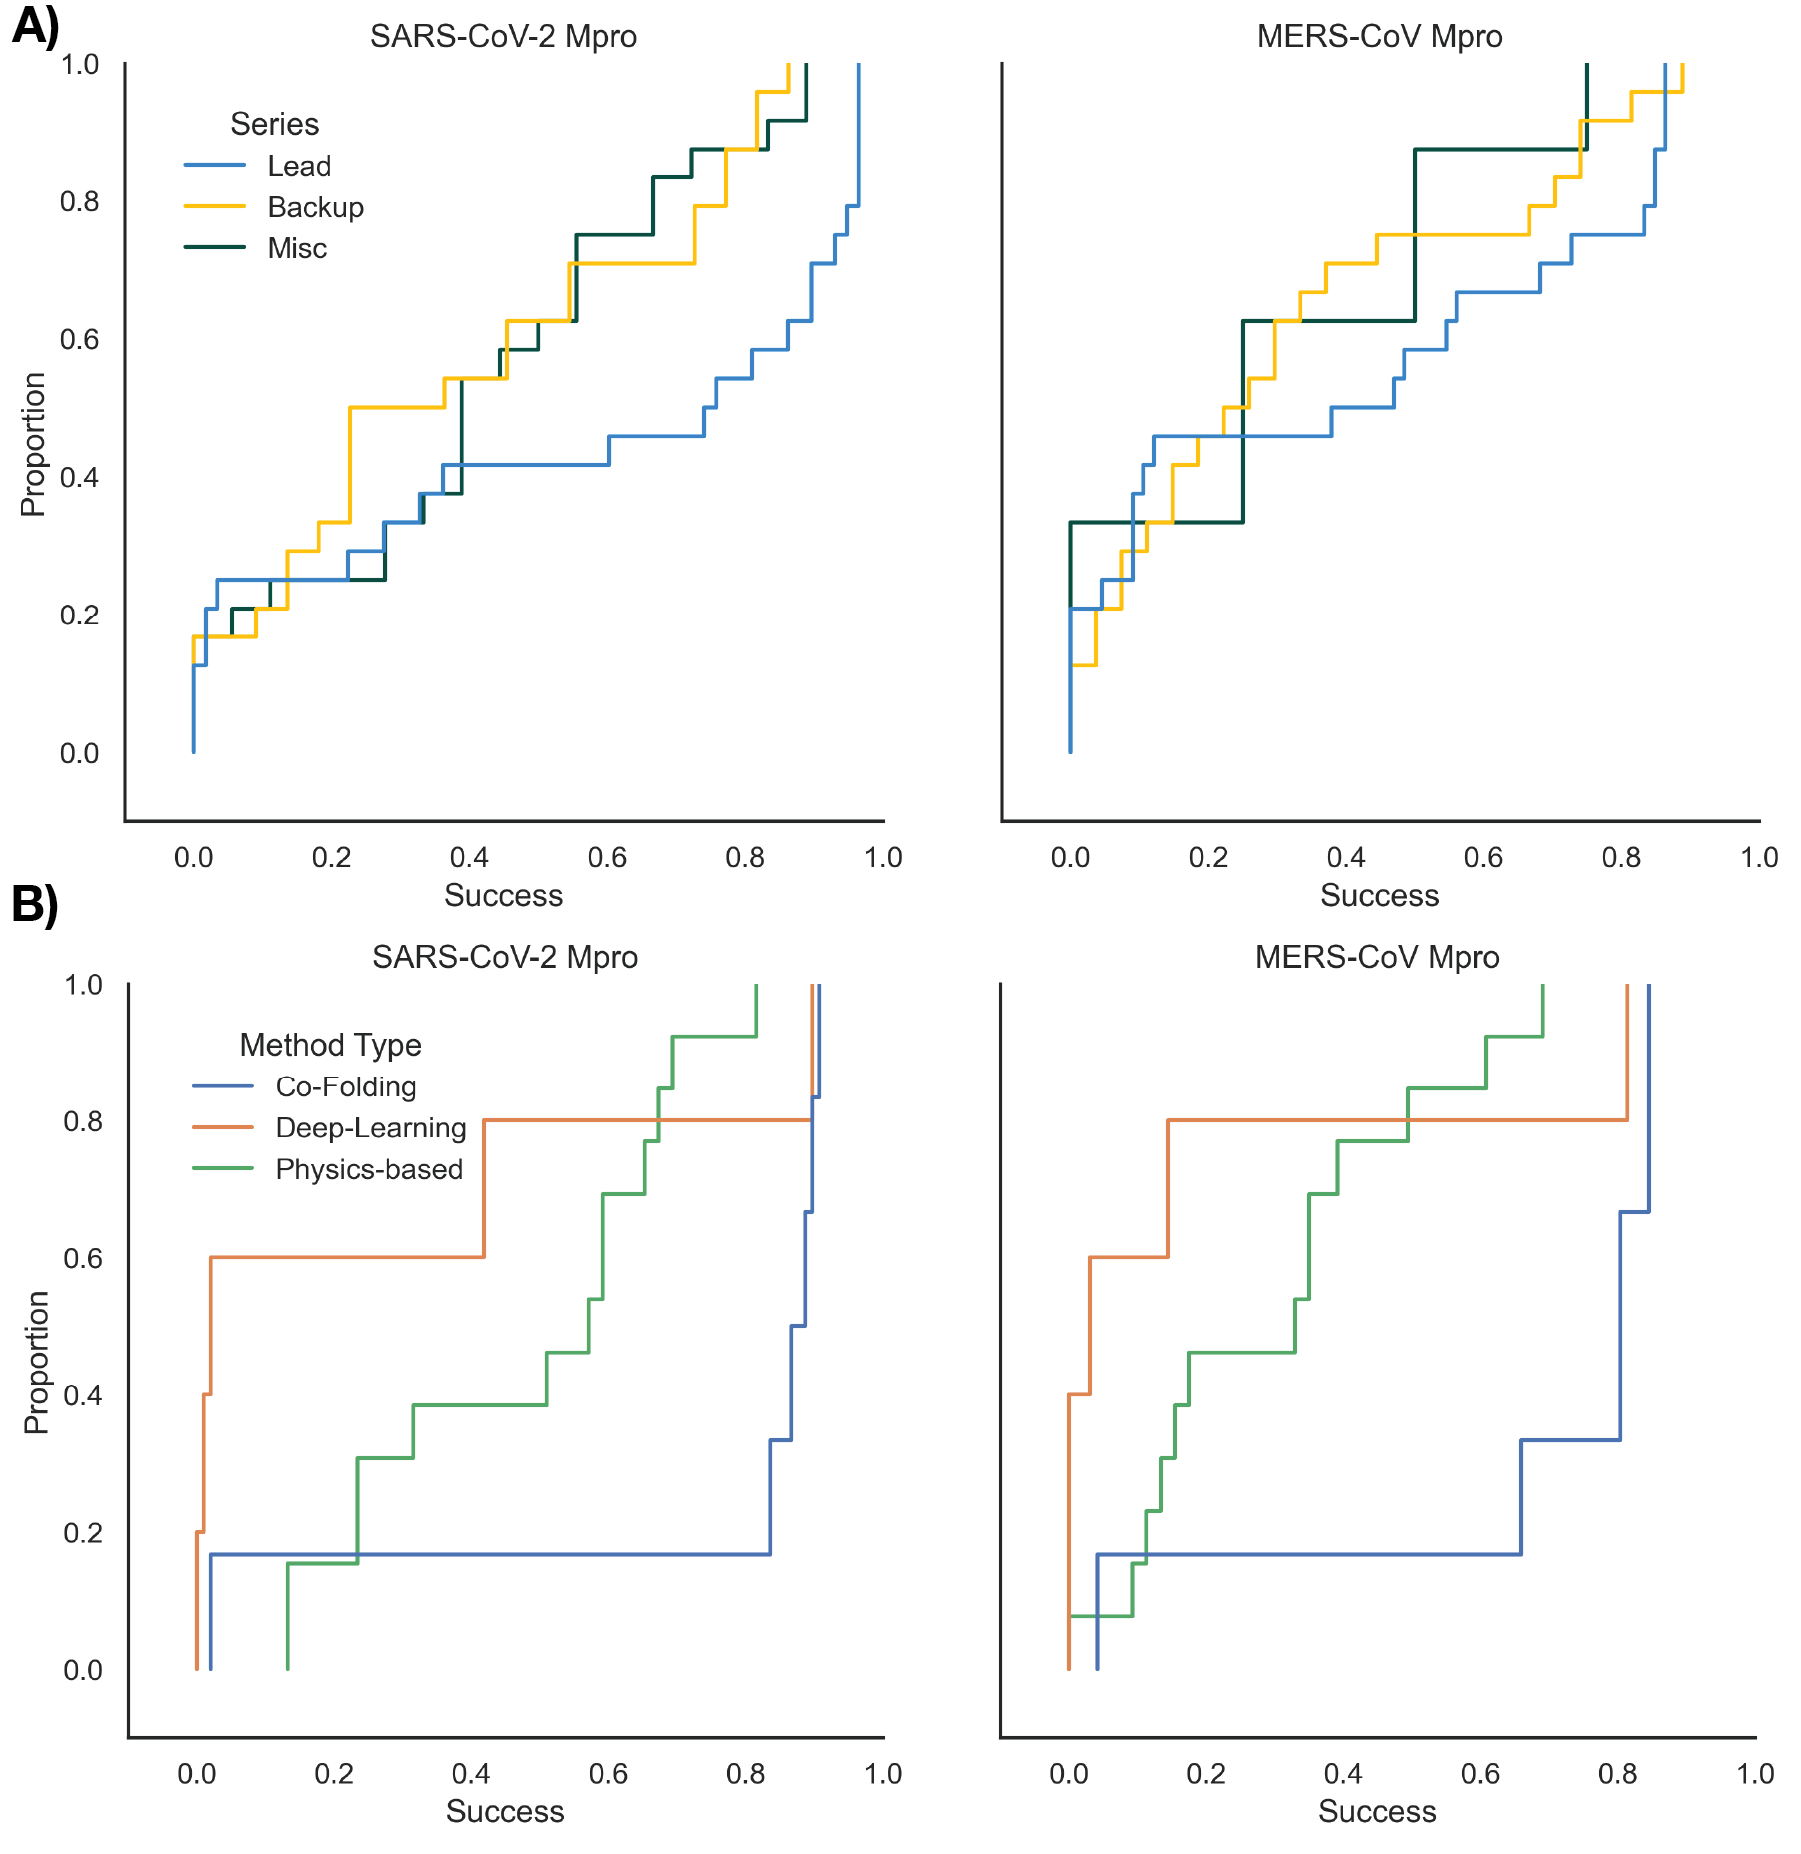
\includegraphics[scale=1
    ]{04_figs_leaderboards/poses_by_series_and_method.png}
  \caption{Participants performed better on the Lead Series than the Backup Series. (A) An empirical cumulative distribution function of the success rates of all the methods for the SARS-CoV-2 (left) or MERS-CoV (right) targets split into either the lead (blue), backup (yellow), or miscellaneous (green) ligand series. Success rates are higher for the lead series than for the backup or miscellaneous series. (B) An empirical cumulative distribution function of the success rates of all the methods for the SARS-CoV-2 (left) or MERS-CoV (right) targets split into their methods types, either co-folding (blue), deep-learning (orange), or physics-based (green). Co-folding methods perform the best, with most models exhibiting a \textgreater 80\% success rate, and deep-learning methods perform the worst, with physics-based methods exhibiting a broad range of success rates.}
  \label{fgr:poses_by_series_and_method}
\end{figure}

Pose-prediction success was evaluated by measuring the fraction of ligands for which the predicted pose had \textless 2 Å symmetry-corrected heavy-atom RMSD from the crystallographic structure. Overall cofolding methods were the most performant, including the top-performing model (\textbf{a}, 82\% success rate), which far outperformed physics-based and deep-learning-based methods in this sub-challenge (Fig. \ref{fgr:poses_leaderboard}). 
Despite only having access to SARS-CoV-2 Mpro data for training, these models performed nearly similarly for the SARS-CoV-2 and MERS-CoV ligand pose predictions. Several possibilities could explain this performance discrepancy. 1) Some models did not employ fine tuning approaches, instead using available co-folding methods "out of the box". 2) fine-tuning on the provided SARS-CoV-2 Mpro training data had little effect on predictive performance, 3) a sufficient amount of SARS-CoV-2 Mpro and MERS-CoV Mpro data were available in the previously publicly available data used to train large cofolding models . 4) SARS-CoV-2 and MERS Mpro are similar enough to each other that co-folding models generalize well between these targets. In depth analysis of these possibilities is beyond the scope of this paper.

By contrast, all but one of the deep-learning-docking methods had low success rates (with many close to a 0\% success rate), with the best performing deep-learning model (\textbf{i}) having a ~20\% success rate for MERS-CoV and a ~40\% success rate for SARS-CoV-2.

Finally, the physics-based methods ranged from ~0\% to ~70\% success, with the best performing physics-based docking method (\textbf{d}) was the reference-based method used by the ASAP Discovery Computational Chemistry team, and the worst performing method was the non-reference-based method provided as a baseline (\textbf{r}). Physics-based methods also showed the greatest discrepancy between the MERS-CoV and SARS-CoV-2 predictions, with a few of the methods showing dramatically better performance for one or the other target. In general, the success rates for SARS-CoV-2 were higher, and the median RMSD for MERS-CoV poses was higher than for SARS-CoV-2. 
The deep learning models (except \textbf{i}) show a surprising reversal of this trend, with the median RMSD for SARS-CoV-2 poses being higher - however the abysmal success rates discourages digging into this too much. 
In conclusion, the \textgreater 80\% success rate of the best-performing co-folding model is quite impressive, and would have hugely benefited the lead optimization of the MERS-CoV series in particular.

This task had a large number of outliers, including conspicuous number of outliers with an RMSD of ~50 Å. We think this is due to the fact that Mpro is a dimer, with most crystal structures containing a ligand bound in both monomers. For this analysis, we just analyzed the chain A ligand, and one of the structures in the dataset had flipped chain A and chain B such that during alignment, the ligand was posed in the second active site. Then, when calculating the RMSD, the ligand is being posed into the wrong active site, making the RMSD anomalously high. Although a meticulous user could have noticed this and corrected the error, we think this was our fault and could have been avoided by either fixing the input structures or enabling users to do their own pose evaluations. Some entries (\textbf{j}, \textbf{m}, \textbf{q}) likely posed their entire series into the wrong chain, resulting in large errors. This kind of error represents the difficulty of working with data from real biological experiments - there are many ways for the data to be misleading to a computer are perfectly valid to the experimentalist.

Figure \ref{fgr:poses_by_series_and_method}

%%%%%%%%%%%%%%%%%%%%%%%%%%%%%%%%%%%%%%%%%%%%%%%%%%%%%%%%%%%%%%%%%%%%%
%% LEARNINGS
%%%%%%%%%%%%%%%%%%%%%%%%%%%%%%%%%%%%%%%%%%%%%%%%%%%%%%%%%%%%%%%%%%%%%
\section{Challenge Key Learnings}


The ASAP-Polaris-OpenADMET blind challenge brought together participants from academia and industry around the globe to showcase cutting-edge approaches in computational methods for drug discovery.

% key takeaways from participants’ results
Key takeaways from the challenge include strong, across-the-board performance of deep learning approaches, with these methods coming first in all three sub-challenges. In the pose prediction sub-challenge, cofolding and cofolding-insipired methods, such as AlphaFold and Boltz, significantly outperformed traditional physics-based approaches, with further improvements observed through fine-tuning. Similarly, in potency prediction, large pretrained deep learning models, especially those based on transformer and graph neural network (GNNs) architectures, were the best performers. For ADMET endpoint prediction, multi-task GNNs proved to be the best approach overall, benefiting from the ability to incorporate auxiliary data.Notably, the top-performing approaches across the three sub-challenges leveraged either additional auxiliary data (public or proprietary) or pre-training outside of the datasets provided by ASAP, highlighting the critical role of data availability in model performance and underscores the need of continuing to expand open and FAIR dataset collection for public benefit. These findings reinforce the value of open initiatives, such as blind challenges, for providing diverse datasets to benchmark and improve existing deep learning models and establishing best practices for predictive methods in drug discovery. Cutting edge open-science projects that may make strides in alleviating this data shortage include US,US and US. 

% Takeaways from challenge execution: Data preparation, Polaris platform, and evaluation metrics
The challenge also offered insight into strategies to successfully execute future public blind challenges. In particular, the detailed data preparation process was essential to prevent data leakage while maintaining chemical diversity, which is essential for preserving real-world model applicability. Dividing the data using a temporal split in the ADMET and potency sub-challenges successfully simulated a prospective drug discovery pipeline, further proving the practical relevance of the results.
Polaris proved to be an ideal platform to host a large number of participants, offering robust feedback mechanisms and enabling streamlined evaluation via a set of standardized metrics. In particular, the Python API provided an intuitive and scalable interface for handling large datasets, which facilitated broad participation. On the other hand, the choice of evaluation metrics allowed for consistent model assessment across different sub-challenges and prediction modalities [??].

[things that weren’t done well and areas of improvement for future challenges]


Data preperation
polaris side:
no user-side eval


%%%%%%%%%%%%%%%%%%%%%%%%%%%%%%%%%%%%%%%%%%%%%%%
%%%%  FROM CAS

% On the scientific value of competitions:
% Competitions are considered the gold standard for unbiased evaluation because...
% They reduce the likelihood of test set leakage.
% They separate method developers from method evaluators (~Goodhart's Law).
% However, just running a competition in itself is not enough. When designing a competition, you need to address three pillars to ensure a competition has real-world impact:
% The competition design (i.e. dataset and evaluation logic) needs to reflect real-world problems.
% Tooling should simplify adoption; It should be easy to do the right thing and hard to do the wrong thing.
% A strong community should foster interdisciplinary collaboration and ensure that lessons learnt are distilled throughout the scientific community.
% In addition to the above, and in an ideal scenario (OpenADMET foreshadowing), a competition is regularly run and updated based on the lessons learnt from previous editions. No one gets it right on the first try and benchmarks should evolve alongside methods.
% All of the above is true for CASP. They didn't just evaluate some methods on blind data, but iteratively refined the Evaluation Logic (e.g. proposed measures of model performance, as well as protein similarity), implemented that evaluation logic in open source software (i.e. OpenStructure), and proactively engaged with the community through papers and conferences to distill the results. I strongly believe this is the key reason the field of structural biology is so mature compared to other domains. CASP has laid and continues to lay the foundation for other benchmarking studies, such as Plinder and Runs 'N Poses.
% On the design of this specific competition:
% Within the context of the above, here are some things about this competition I think we did well:
% Unbiased evaluation: Performance on the test set was only measured three times.
% Unbiased evaluation: Performance was evaluated by an independent team.
% Real-world impact: Dataset stems from a real drug discovery program.
% Real-world impact: Use of bootstrapping, statistical testing and CLD, based on this.
% Real-world impact: We report many performance metrics, both on a task and aggregate level.
% Real-world impact: Inclusion of baselines to contextualize the results.
% Real-world impact: More granular, detailed analysis in this paper to understand utility of best performing methods. When do these models succeed and when do they fail?
% Ease of use: Pythonic API
% Ease of use: ML-ready datasets, with access to the raw data.
% Scientific community: We're submitting results to a special issue at JCIM.
% Scientific community: We organized office hours.
% Scientific community: Report required from each final submissions.
% Scientific community: Low barrier for communication with organizers and other participants through Discord.
% Scientific community: We organized webinars to discuss final results.
% Scientific community: Dataset was unblinded after the competition.
% Scientific community: Evaluation logic was open-sourced after the competition.
% %%%%%%%%%%%%%%%%%%%%%%%%%%%%%%%%%%%%%%%%%%%%%%%%


\subsection{The future of blind challenges}

% Outlook for future challenges
We believe that blind challenges are the best way to robustly assess models and drive forward computational methods in drug discovery. This is validated by step-change improvements in model performance after community investment in blind challenges both in related fields such as computer vision (XX and XX), natural language processing (XX and XX) and abstract reasoning (XX and XX), and in those relevant to drug discovery such as computational structure prediction (CASP). Infrastructure like Polaris can help make blind challenges more routine, consistent and with operate with lower overhead. XXXXX


%%%%%%%%%%%%%%%%%%%%%%%%%%%%%%%%%%%%%%%%%%%%%%%%%%%%%%%%%%%%%%%%%%%%%
%% The "Acknowledgement" section can be given in all manuscript
%% classes.  This should be given within the "acknowledgement"
%% environment, which will make the correct section or running title.
%%%%%%%%%%%%%%%%%%%%%%%%%%%%%%%%%%%%%%%%%%%%%%%%%%%%%%%%%%%%%%%%%%%%%
\begin{acknowledgement}

Please use ``The authors thank \ldots'' rather than ``The
authors would like to thank \ldots''.

\end{acknowledgement}

%%%%%%%%%%%%%%%%%%%%%%%%%%%%%%%%%%%%%%%%%%%%%%%%%%%%%%%%%%%%%%%%%%%%%
%% The same is true for Supporting Information, which should use the
%% suppinfo environment.
%%%%%%%%%%%%%%%%%%%%%%%%%%%%%%%%%%%%%%%%%%%%%%%%%%%%%%%%%%%%%%%%%%%%%
\begin{suppinfo}

Additional analyses to support main conclusions. 

\end{suppinfo}

%%%%%%%%%%%%%%%%%%%%%%%%%%%%%%%%%%%%%%%%%%%%%%%%%%%%%%%%%%%%%%%%%%%%%
%% The appropriate \bibliography command should be placed here.
%% Notice that the class file automatically sets \bibliographystyle
%% and also names the section correctly.
%%%%%%%%%%%%%%%%%%%%%%%%%%%%%%%%%%%%%%%%%%%%%%%%%%%%%%%%%%%%%%%%%%%%%
\bibliography{references}

\end{document}